%%% IMPORTANTE: Compilar no Overleaf usando o template SBC
%%% Template: https://www.overleaf.com/gallery/tagged/sbc
%%% Copie este arquivo para o projeto Overleaf junto com sbc-template.sty

\documentclass[12pt]{article}

\usepackage{sbc-template}
\usepackage{graphicx}
\usepackage{url}
\usepackage[brazil]{babel}
\usepackage[utf8]{inputenc}
\usepackage[T1]{fontenc}
\usepackage{booktabs}
\usepackage{multirow}
\usepackage{amsmath}
\usepackage{float}
\usepackage{caption}
\usepackage{subcaption}
\usepackage{hyperref}
\usepackage{array}
\usepackage{xcolor}
\usepackage{siunitx}

\hypersetup{
    colorlinks=true,
    linkcolor=blue,
    urlcolor=blue,
    citecolor=blue
}

% ── Metadados ─────────────────────────────────────────────────
\sloppy

\title{Análise Estatística de Métricas de Código-Fonte do Framework JUnit}

\author{
  João Pedro Giovanelli\inst{1},
  Enzo Perroni\inst{1}
}

\address{
  Curso de Engenharia de Software -- IBMEC\\
  Rio de Janeiro, RJ, Brasil
  \email{joaopedrogiovanelli@gmail.com, zocaperroni@gmail.com}
}

% ═══════════════════════════════════════════════════════════════
\begin{document}

\maketitle

% ── Resumo ────────────────────────────────────────────────────
\begin{abstract}
This paper presents a comprehensive statistical analysis of source code
metrics from the Java testing framework \textbf{JUnit}, using data from
the \textit{GitHub Bug Dataset} version~1.1. From a set of 1,154 Java
classes, we selected ten representative metrics — covering complexity,
coupling, cohesion, inheritance, size, quality, and documentation — and
applied descriptive and inferential statistical techniques: measures of
central tendency and dispersion, quartile analysis, chart construction,
outlier detection, normality tests (Shapiro-Wilk and Kolmogorov-Smirnov),
correlation analysis (Pearson and Spearman), and statistical modeling
(multiple linear regression and logistic regression). Results reveal
strong positive skewness across all metrics, universal non-normality, and
a high-correlation cluster among lines of code (LOC), weighted methods per
class (WMC), and response for a class (RFC). Depth of inheritance tree
(DIT) proved statistically independent of all other variables. The multiple
linear regression model explains 34\% of WMC variability without LOC
(avoiding multicollinearity), while the logistic model achieves an
AUC-ROC of 0.744 for predicting the presence of severe PMD warnings. The
full source code and dataset are available at:
\url{https://github.com/jpgiovanelli/ibmec.proj_es}.
\end{abstract}

\begin{resumo}
Este artigo apresenta uma análise estatística abrangente de métricas de
código-fonte do framework de testes Java \textbf{JUnit}, utilizando dados
provenientes do \textit{GitHub Bug Dataset} versão~1.1. A partir de um
conjunto de 1.154 classes Java, selecionamos dez métricas representativas
— cobrindo complexidade, acoplamento, coesão, herança, tamanho, qualidade
e documentação — e aplicamos técnicas de estatística descritiva e
inferencial: medidas de tendência central e dispersão, análise de quartis,
construção de gráficos, detecção de outliers, testes de normalidade
(Shapiro-Wilk e Kolmogorov-Smirnov), análise de correlação (Pearson e
Spearman) e modelagem estatística (regressão linear múltipla e regressão
logística). Os resultados revelam forte assimetria positiva em todas as
métricas, não-normalidade universal, e um cluster de alta correlação entre
linhas de código (LOC), complexidade ciclomática ponderada (WMC) e resposta
por classe (RFC). A profundidade de herança (DIT) mostrou-se
estatisticamente independente das demais variáveis. O modelo de regressão
linear múltipla explica 34\% da variabilidade de WMC sem uso de LOC
(evitando multicolinearidade), enquanto o modelo logístico atinge
AUC-ROC de 0,744 na predição de presença de avisos PMD severos. O
código-fonte completo e o conjunto de dados estão disponíveis em:
\url{https://github.com/jpgiovanelli/ibmec.proj_es}.
\end{resumo}

% ═══════════════════════════════════════════════════════════════
\section{Introdução}
\label{sec:intro}

A qualidade do software é uma preocupação central da Engenharia de
Software moderna. Métricas de código-fonte constituem instrumentos
objetivos para avaliar características estruturais de sistemas,
identificar componentes problemáticos e orientar decisões de
refatoração~\cite{chidamber1994}. Em particular, métricas orientadas
a objetos — como WMC, CBO, DIT e LCOM — têm sido amplamente
estudadas em sua relação com defeitos, manutenibilidade e
complexidade~\cite{briand1999}.

O \textbf{JUnit} é um dos frameworks de teste mais utilizados no
ecossistema Java, com décadas de desenvolvimento comunitário ativo.
Sua análise estática fornece um caso de estudo representativo de
software de produção bem consolidado. Este trabalho aplica técnicas
de estatística descritiva e inferencial ao dataset de métricas de
código-fonte do JUnit, disponibilizado pelo \textit{GitHub Bug
Dataset}~\cite{Ferenc2020}, com os seguintes objetivos:

\begin{enumerate}
  \item Caracterizar estatisticamente as métricas de código do JUnit;
  \item Identificar padrões de correlação entre métricas;
  \item Avaliar a não-normalidade e a presença de outliers;
  \item Construir modelos preditivos para complexidade e qualidade de código.
\end{enumerate}

O restante do artigo está organizado como segue: a Seção~\ref{sec:metodologia}
descreve o dataset e o método analítico; a Seção~\ref{sec:resultados}
apresenta os resultados; a Seção~\ref{sec:discussao} discute os
achados; a Seção~\ref{sec:conclusao} conclui o trabalho.

% ═══════════════════════════════════════════════════════════════
\section{Metodologia}
\label{sec:metodologia}

\subsection{Fonte de Dados}

O dataset utilizado é o \textit{GitHub Bug Dataset} versão~1.1,
disponibilizado por \cite{Ferenc2020}. Para o framework JUnit,
estão disponíveis dois arquivos CSV correspondentes a versões
distintas do projeto: \texttt{junit-File.csv} (métricas em nível
de arquivo) e \texttt{junit-Class.csv} (métricas em nível de
classe). Seguindo as diretrizes do trabalho, utilizamos o dataset
mais recente — \texttt{junit-Class.csv}.

\subsection{Descrição do Dataset}

O arquivo \texttt{junit-Class.csv} contém \textbf{1.154 observações}
(classes Java, incluindo classes internas e anônimas) e \textbf{113
colunas}, sendo 6 identificadoras (ID, nome, caminho) e 107 numéricas.
As colunas numéricas abrangem: métricas orientadas a objetos,
métricas de tamanho, métricas de clone, indicadores de documentação,
contagens de avisos de ferramentas estáticas (PMD) e a variável alvo
``\textit{Number of bugs}''.

\textbf{Limitação crítica:} A variável ``\textit{Number of bugs}'' apresenta
valor zero em todas as 1.154 observações, impossibilitando seu uso direto
como variável resposta em modelos de regressão. Esse resultado é
consistente com a maturidade do JUnit enquanto framework de teste amplamente
auditado pela comunidade. Diante disso, adotamos como variável resposta
principal o WMC (regressão linear) e uma variável binária derivada de
WarningMajor (regressão logística), conforme detalhado na
Seção~\ref{sec:modelagem}.

\subsection{Seleção de Variáveis}

Foram selecionadas \textbf{dez variáveis numéricas} com base em quatro
critérios: (i) variância não-nula, (ii) interpretabilidade no contexto
de Engenharia de Software, (iii) diversidade de distribuições e
(iv) baixa redundância entre si. A Tabela~\ref{tab:variaveis} descreve
as variáveis selecionadas.

\begin{table}[H]
\centering
\caption{Variáveis selecionadas para análise}
\label{tab:variaveis}
\begin{tabular}{llp{6cm}}
\toprule
\textbf{Variável} & \textbf{Tipo} & \textbf{Descrição} \\
\midrule
WMC          & int   & \textit{Weighted Methods per Class} — complexidade ponderada \\
CBO          & int   & \textit{Coupling Between Objects} — acoplamento \\
LCOM5        & float & \textit{Lack of Cohesion of Methods} — falta de coesão \\
DIT          & int   & \textit{Depth of Inheritance Tree} — profundidade de herança \\
RFC          & int   & \textit{Response for a Class} — tamanho do conjunto de resposta \\
LOC          & int   & \textit{Lines of Code} — tamanho do código \\
NM           & int   & \textit{Number of Methods} — número de métodos \\
WarningInfo  & int   & Avisos PMD informativos \\
WarningMajor & int   & Avisos PMD severos \\
CD           & float & \textit{Comment Density} — densidade de comentários \\
\bottomrule
\end{tabular}
\end{table}

\subsection{Ferramentas e Ambiente}

A análise foi conduzida em duas linguagens:
\begin{itemize}
  \item \textbf{Python 3.12:} pacotes \texttt{pandas}, \texttt{numpy},
        \texttt{scipy}, \texttt{matplotlib}, \texttt{seaborn} e
        \texttt{statsmodels}, para exploração inicial e validação;
  \item \textbf{R 4.x:} pacotes \texttt{ggplot2}, \texttt{dplyr},
        \texttt{PerformanceAnalytics}, \texttt{car}, \texttt{nortest}
        e \texttt{pROC}, para análise definitiva.
\end{itemize}

Todo o código e os dados estão disponíveis em:
\url{https://github.com/jpgiovanelli/ibmec.proj_es}.

% ═══════════════════════════════════════════════════════════════
\section{Resultados}
\label{sec:resultados}

\subsection{Medidas de Tendência Central}
\label{sec:central}

A Tabela~\ref{tab:central} apresenta as medidas de tendência central
para as dez variáveis selecionadas.

\begin{table}[H]
\centering
\caption{Medidas de tendência central}
\label{tab:central}
\begin{tabular}{lrrr}
\toprule
\textbf{Variável} & \textbf{Média} & \textbf{Mediana} & \textbf{Moda} \\
\midrule
WMC          & 4,05  & 2,0  & 1,0 \\
CBO          & 3,81  & 3,0  & 2,0 \\
LCOM5        & 1,68  & 1,0  & 1,0 \\
DIT          & 0,55  & 0,0  & 0,0 \\
RFC          & 5,26  & 2,0  & 1,0 \\
LOC          & 26,95 & 11,0 & 6,0 \\
NM           & 11,35 & 2,0  & 1,0 \\
WarningInfo  & 16,58 & 9,0  & 5,0 \\
WarningMajor & 1,43  & 0,0  & 0,0 \\
CD           & 0,064 & 0,0  & 0,0 \\
\bottomrule
\end{tabular}
\end{table}

Em todas as variáveis, a média é consideravelmente superior à mediana,
evidenciando forte assimetria positiva — característica típica de
métricas de software, onde poucas classes grandes dominam a distribuição.
Para CD e WarningMajor, a mediana e a moda são zero, indicando
\textit{zero-inflation}: a maioria das classes não possui documentação
por comentários ou violações PMD severas.

\subsection{Medidas de Dispersão}
\label{sec:dispersao}

A Tabela~\ref{tab:dispersao} apresenta as medidas de dispersão.
Destaca-se que todos os coeficientes de variação (CV) superam 100\%,
confirmando a heterogeneidade extrema do dataset. WarningMajor e CD
apresentam os maiores CV (266\% e 250\%, respectivamente), refletindo
a distribuição altamente concentrada em zero com caudas pesadas à direita.

\begin{table}[H]
\centering
\caption{Medidas de dispersão}
\label{tab:dispersao}
\begin{tabular}{lrrrr}
\toprule
\textbf{Variável} & \textbf{Amplitude} & \textbf{Variância} & \textbf{Desvio Padrão} & \textbf{CV (\%)} \\
\midrule
WMC          & 108   & 65,5    & 8,10  & 199,9 \\
CBO          & 106   & 23,9    & 4,89  & 128,2 \\
LCOM5        & 78    & 10,9    & 3,31  & 196,7 \\
DIT          & 5     & 0,75    & 0,87  & 159,2 \\
RFC          & 115   & 77,5    & 8,80  & 167,5 \\
LOC          & 934   & 2891,3  & 53,77 & 199,5 \\
NM           & 118   & 600,7   & 24,51 & 215,9 \\
WarningInfo  & 567   & 991,6   & 31,49 & 189,9 \\
WarningMajor & 85    & 14,5    & 3,81  & 265,9 \\
CD           & 0,923 & 0,026   & 0,160 & 250,3 \\
\bottomrule
\end{tabular}
\end{table}

\subsection{Medidas de Posição Relativa e Boxplots}
\label{sec:posicao}

A Figura~\ref{fig:boxplots} apresenta os boxplots das dez variáveis.
A grande quantidade de outliers visíveis acima do limite superior de cada
caixa confirma a assimetria já observada.

\begin{figure}[H]
  \centering
  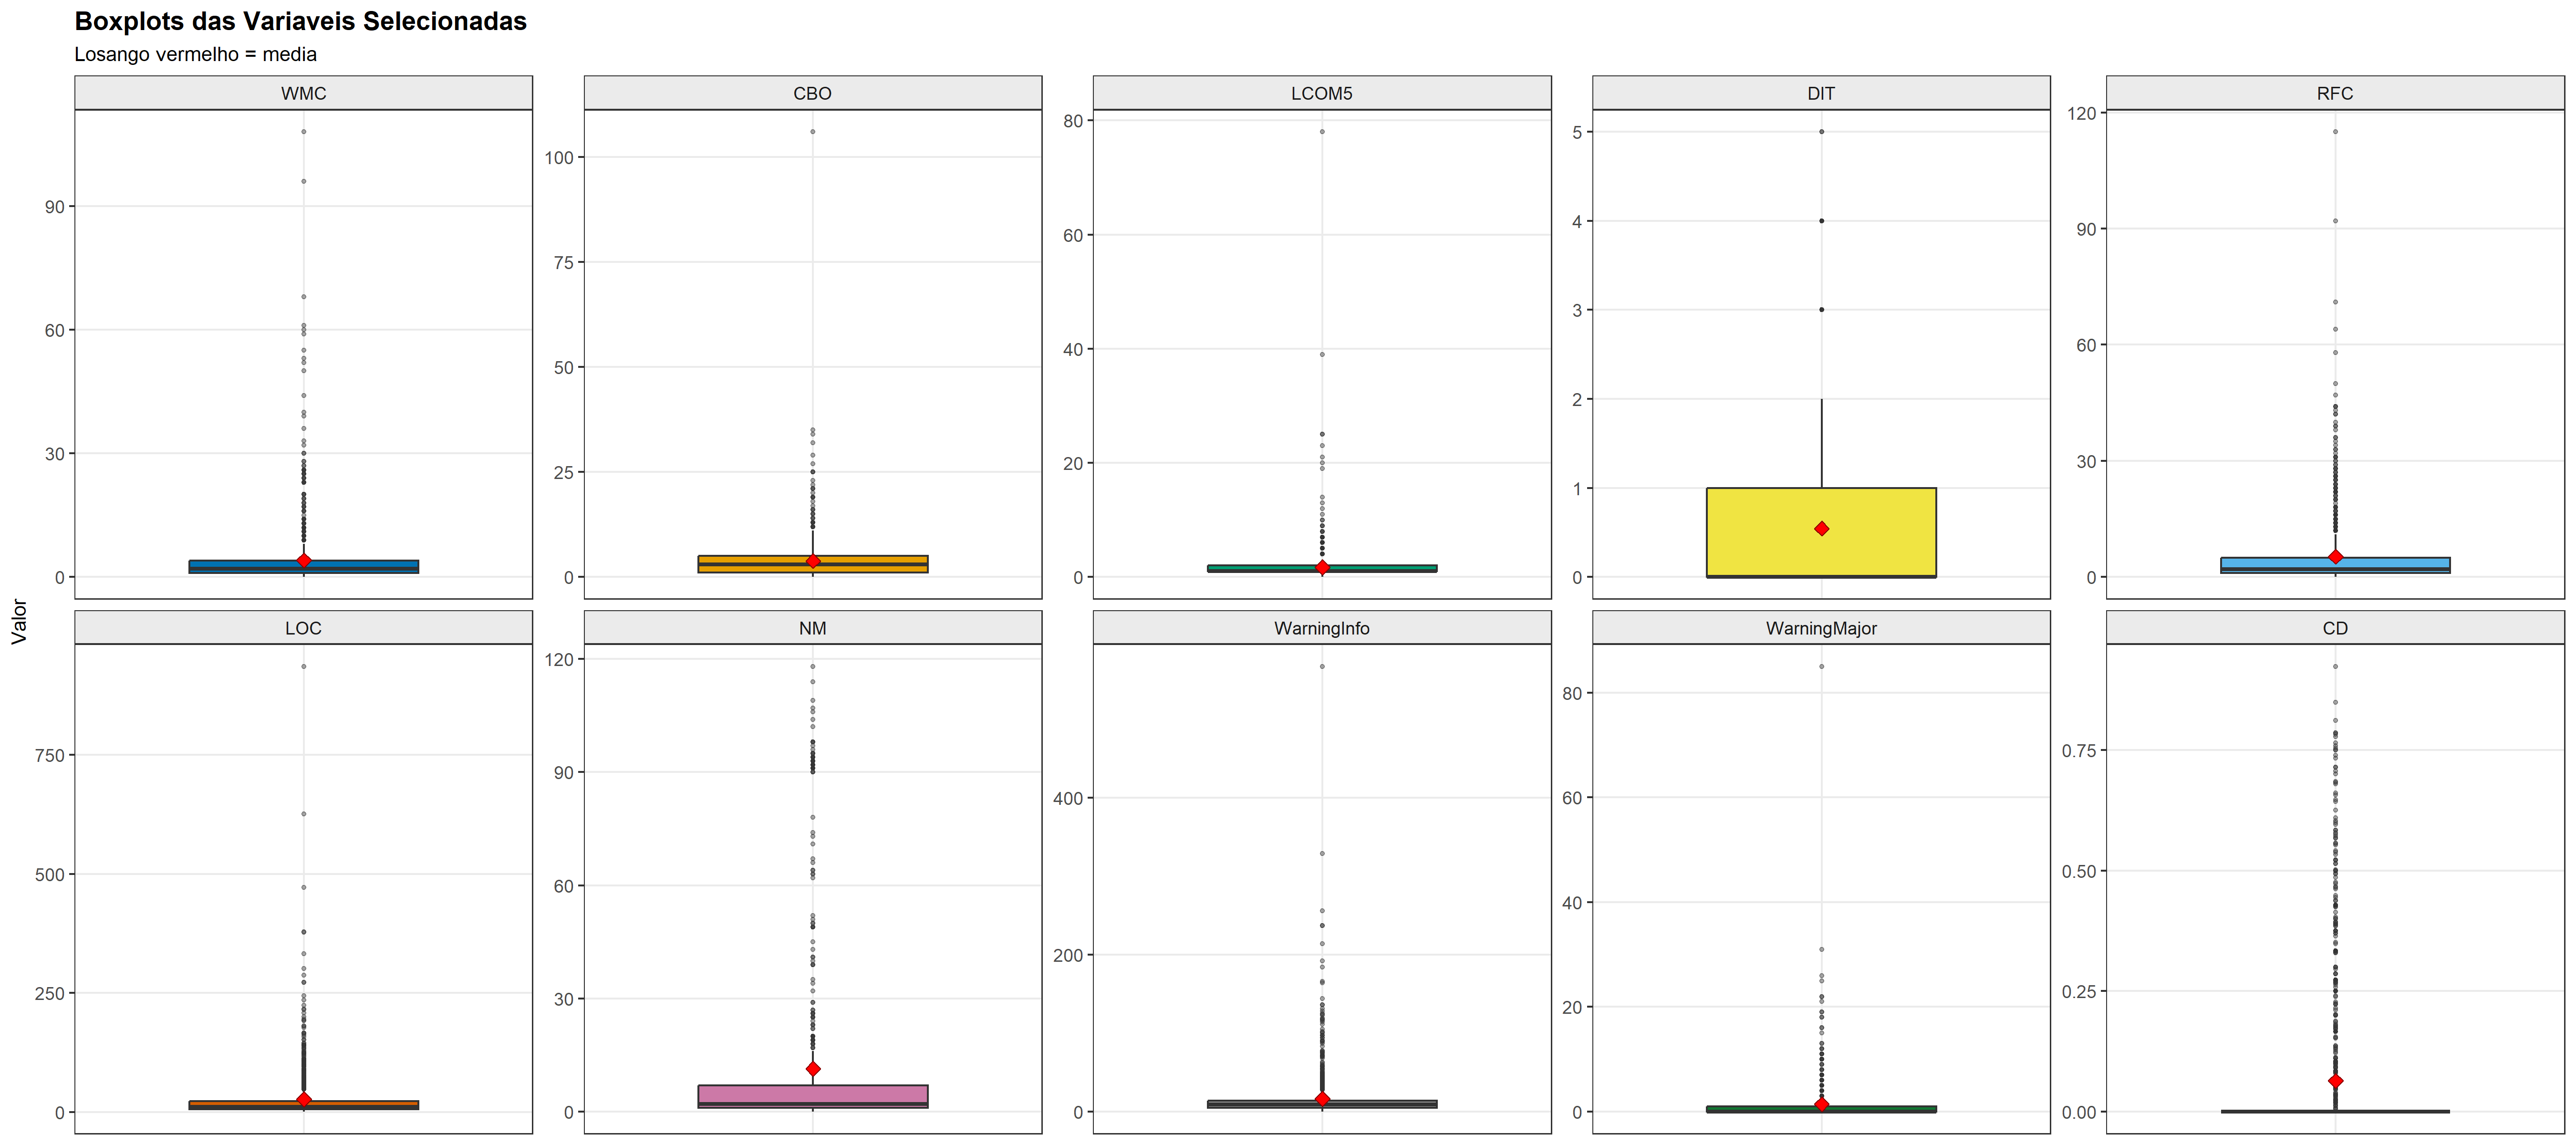
\includegraphics[width=\linewidth]{../output/figures_r/boxplots_all_r.png}
  \caption{Boxplots das variáveis selecionadas. O losango vermelho indica a média.}
  \label{fig:boxplots}
\end{figure}

A Tabela~\ref{tab:percentis} apresenta os percentis e o IQR para cada
variável. Para DIT, o terceiro quartil é 1 e o máximo é 5, refletindo
que a grande maioria das classes do JUnit possui herança rasa ou nenhuma.

\begin{table}[H]
\centering
\caption{Percentis selecionados e IQR}
\label{tab:percentis}
\begin{tabular}{lrrrrrrrr}
\toprule
\textbf{Var.} & \textbf{P5} & \textbf{Q1} & \textbf{Med.} & \textbf{Q3} & \textbf{P90} & \textbf{P95} & \textbf{IQR} \\
\midrule
WMC          & 0    & 1    & 2     & 4,00  & 9,0  & 16,0   & 3,00 \\
CBO          & 0    & 1    & 3     & 5,00  & 8,0  & 10,0   & 4,00 \\
LCOM5        & 0    & 1    & 1     & 2,00  & 3,0  & 5,0    & 1,00 \\
DIT          & 0    & 0    & 0     & 1,00  & 2,0  & 2,0    & 1,00 \\
RFC          & 0    & 1    & 2     & 5,00  & 12,0 & 22,0   & 4,00 \\
LOC          & 3    & 6    & 11    & 22,75 & 64,7 & 109,4  & 16,75\\
NM           & 0    & 1    & 2     & 7,00  & 26,0 & 91,0   & 6,00 \\
WarningInfo  & 3    & 5    & 9     & 14,00 & 33,0 & 58,0   & 9,00 \\
WarningMajor & 0    & 0    & 0     & 1,00  & 4,0  & 6,0    & 1,00 \\
CD           & 0    & 0    & 0     & 0,00  & 0,27 & 0,47   & 0,00 \\
\bottomrule
\end{tabular}
\end{table}

\subsection{Análise Gráfica}
\label{sec:graficos}

\subsubsection{Histogramas}

A Figura~\ref{fig:histogramas} confirma visualmente a assimetria positiva
e a \textit{zero-inflation}. Para todas as variáveis, a curva de densidade
exibe cauda longa à direita; a média (linha vermelha tracejada) é
sistematicamente deslocada para a direita da mediana (linha verde).

\begin{figure}[H]
  \centering
  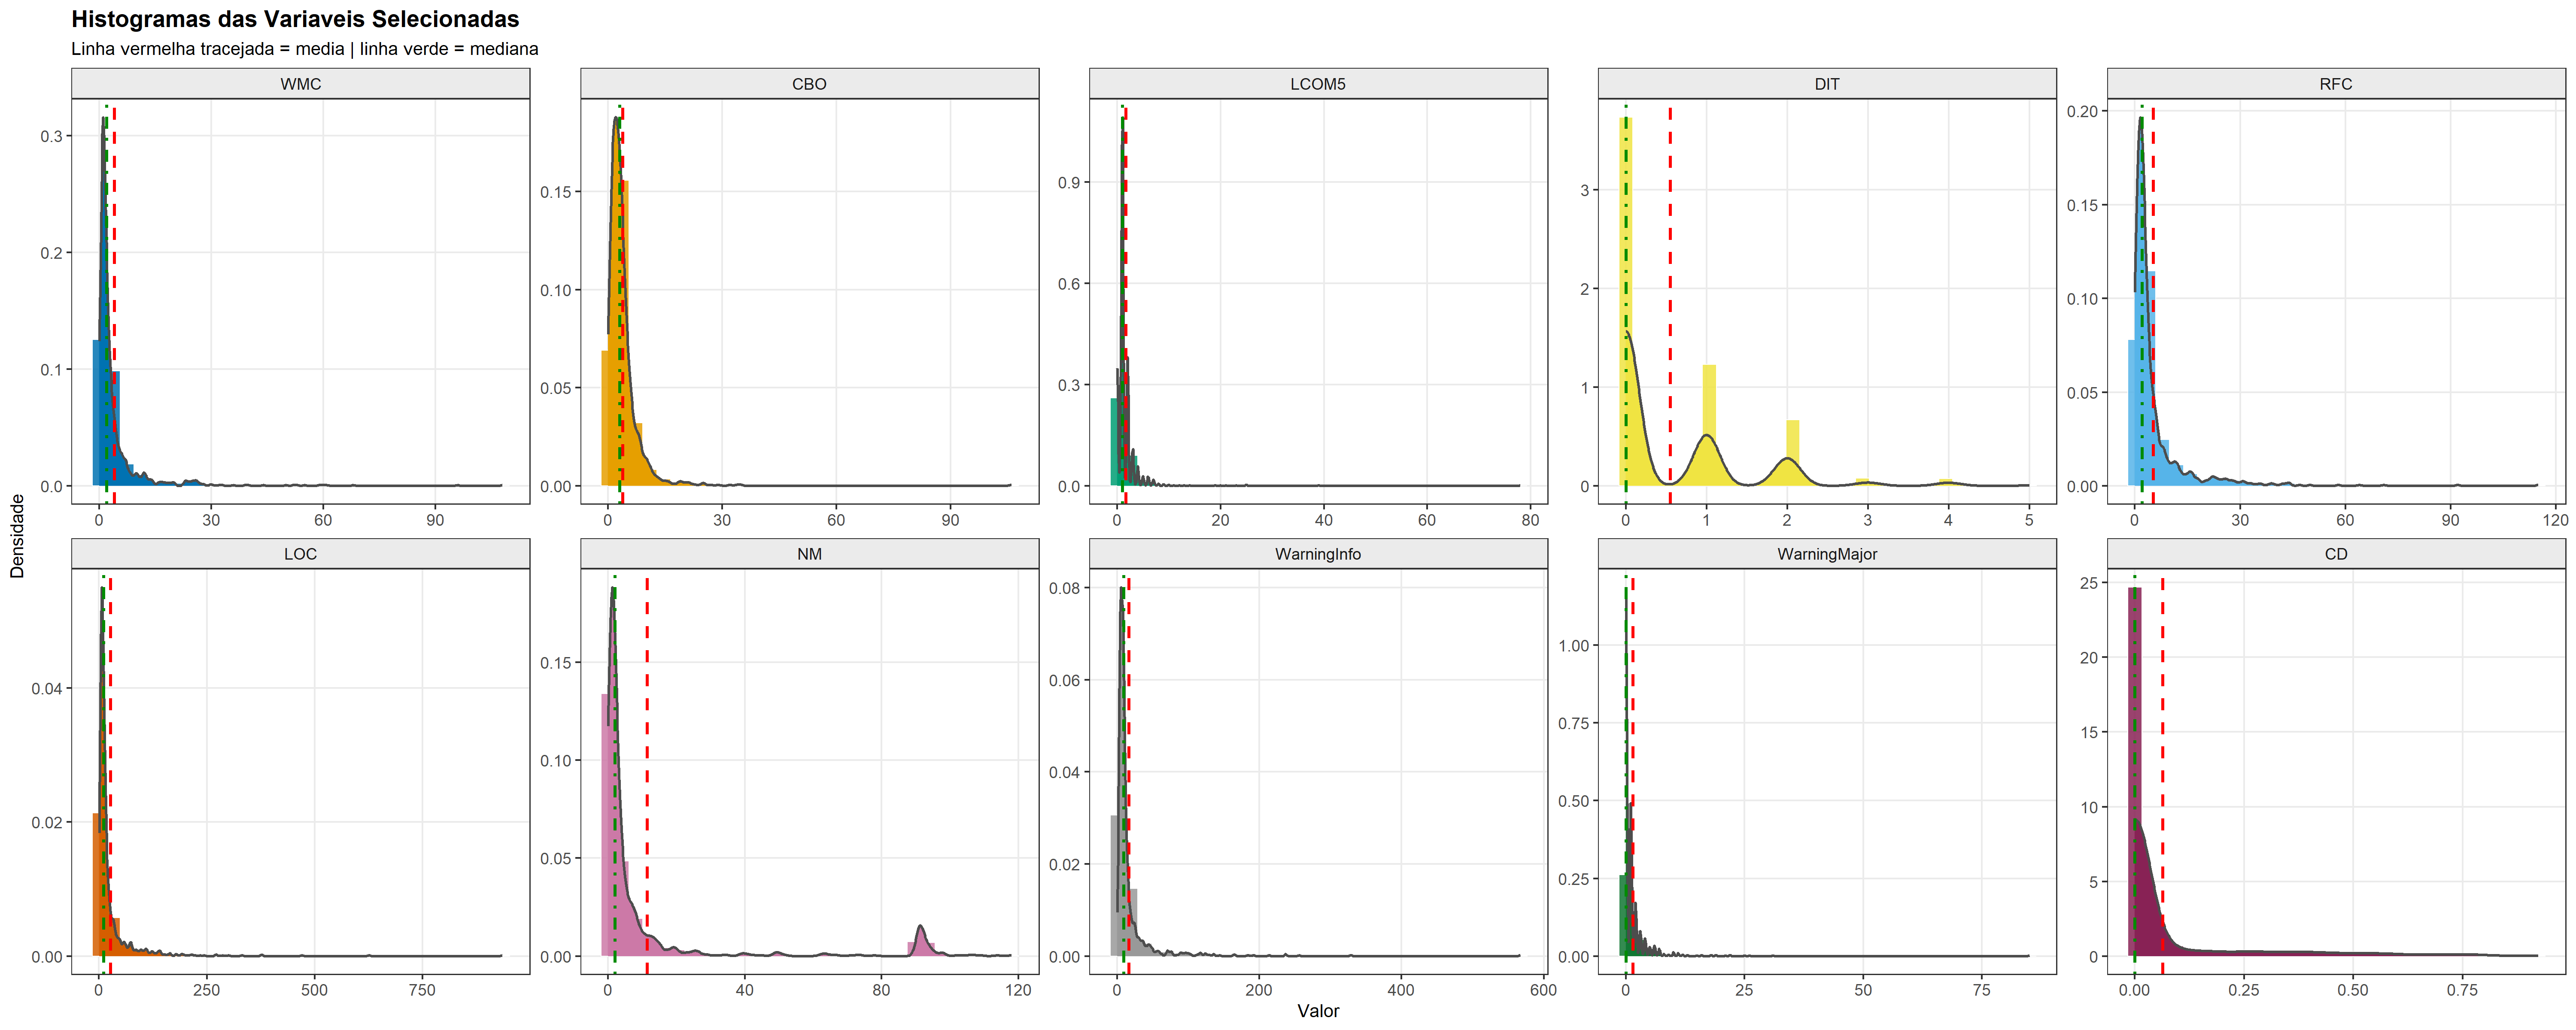
\includegraphics[width=\linewidth]{../output/figures_r/histograms_r.png}
  \caption{Histogramas com estimativa de densidade e linhas de média/mediana.}
  \label{fig:histogramas}
\end{figure}

\subsubsection{Gráficos de Dispersão}

A Figura~\ref{fig:scatter} apresenta seis pares de variáveis com linhas
de regressão e coeficientes de Pearson ($r$) e Spearman ($\rho$) anotados.
Destaca-se a forte linearidade entre LOC e WMC ($r = 0{,}94$) e entre
LOC e RFC ($r = 0{,}90$), enquanto o par DIT × CBO revela correlação
próxima de zero ($r = -0{,}05$).

\begin{figure}[H]
  \centering
  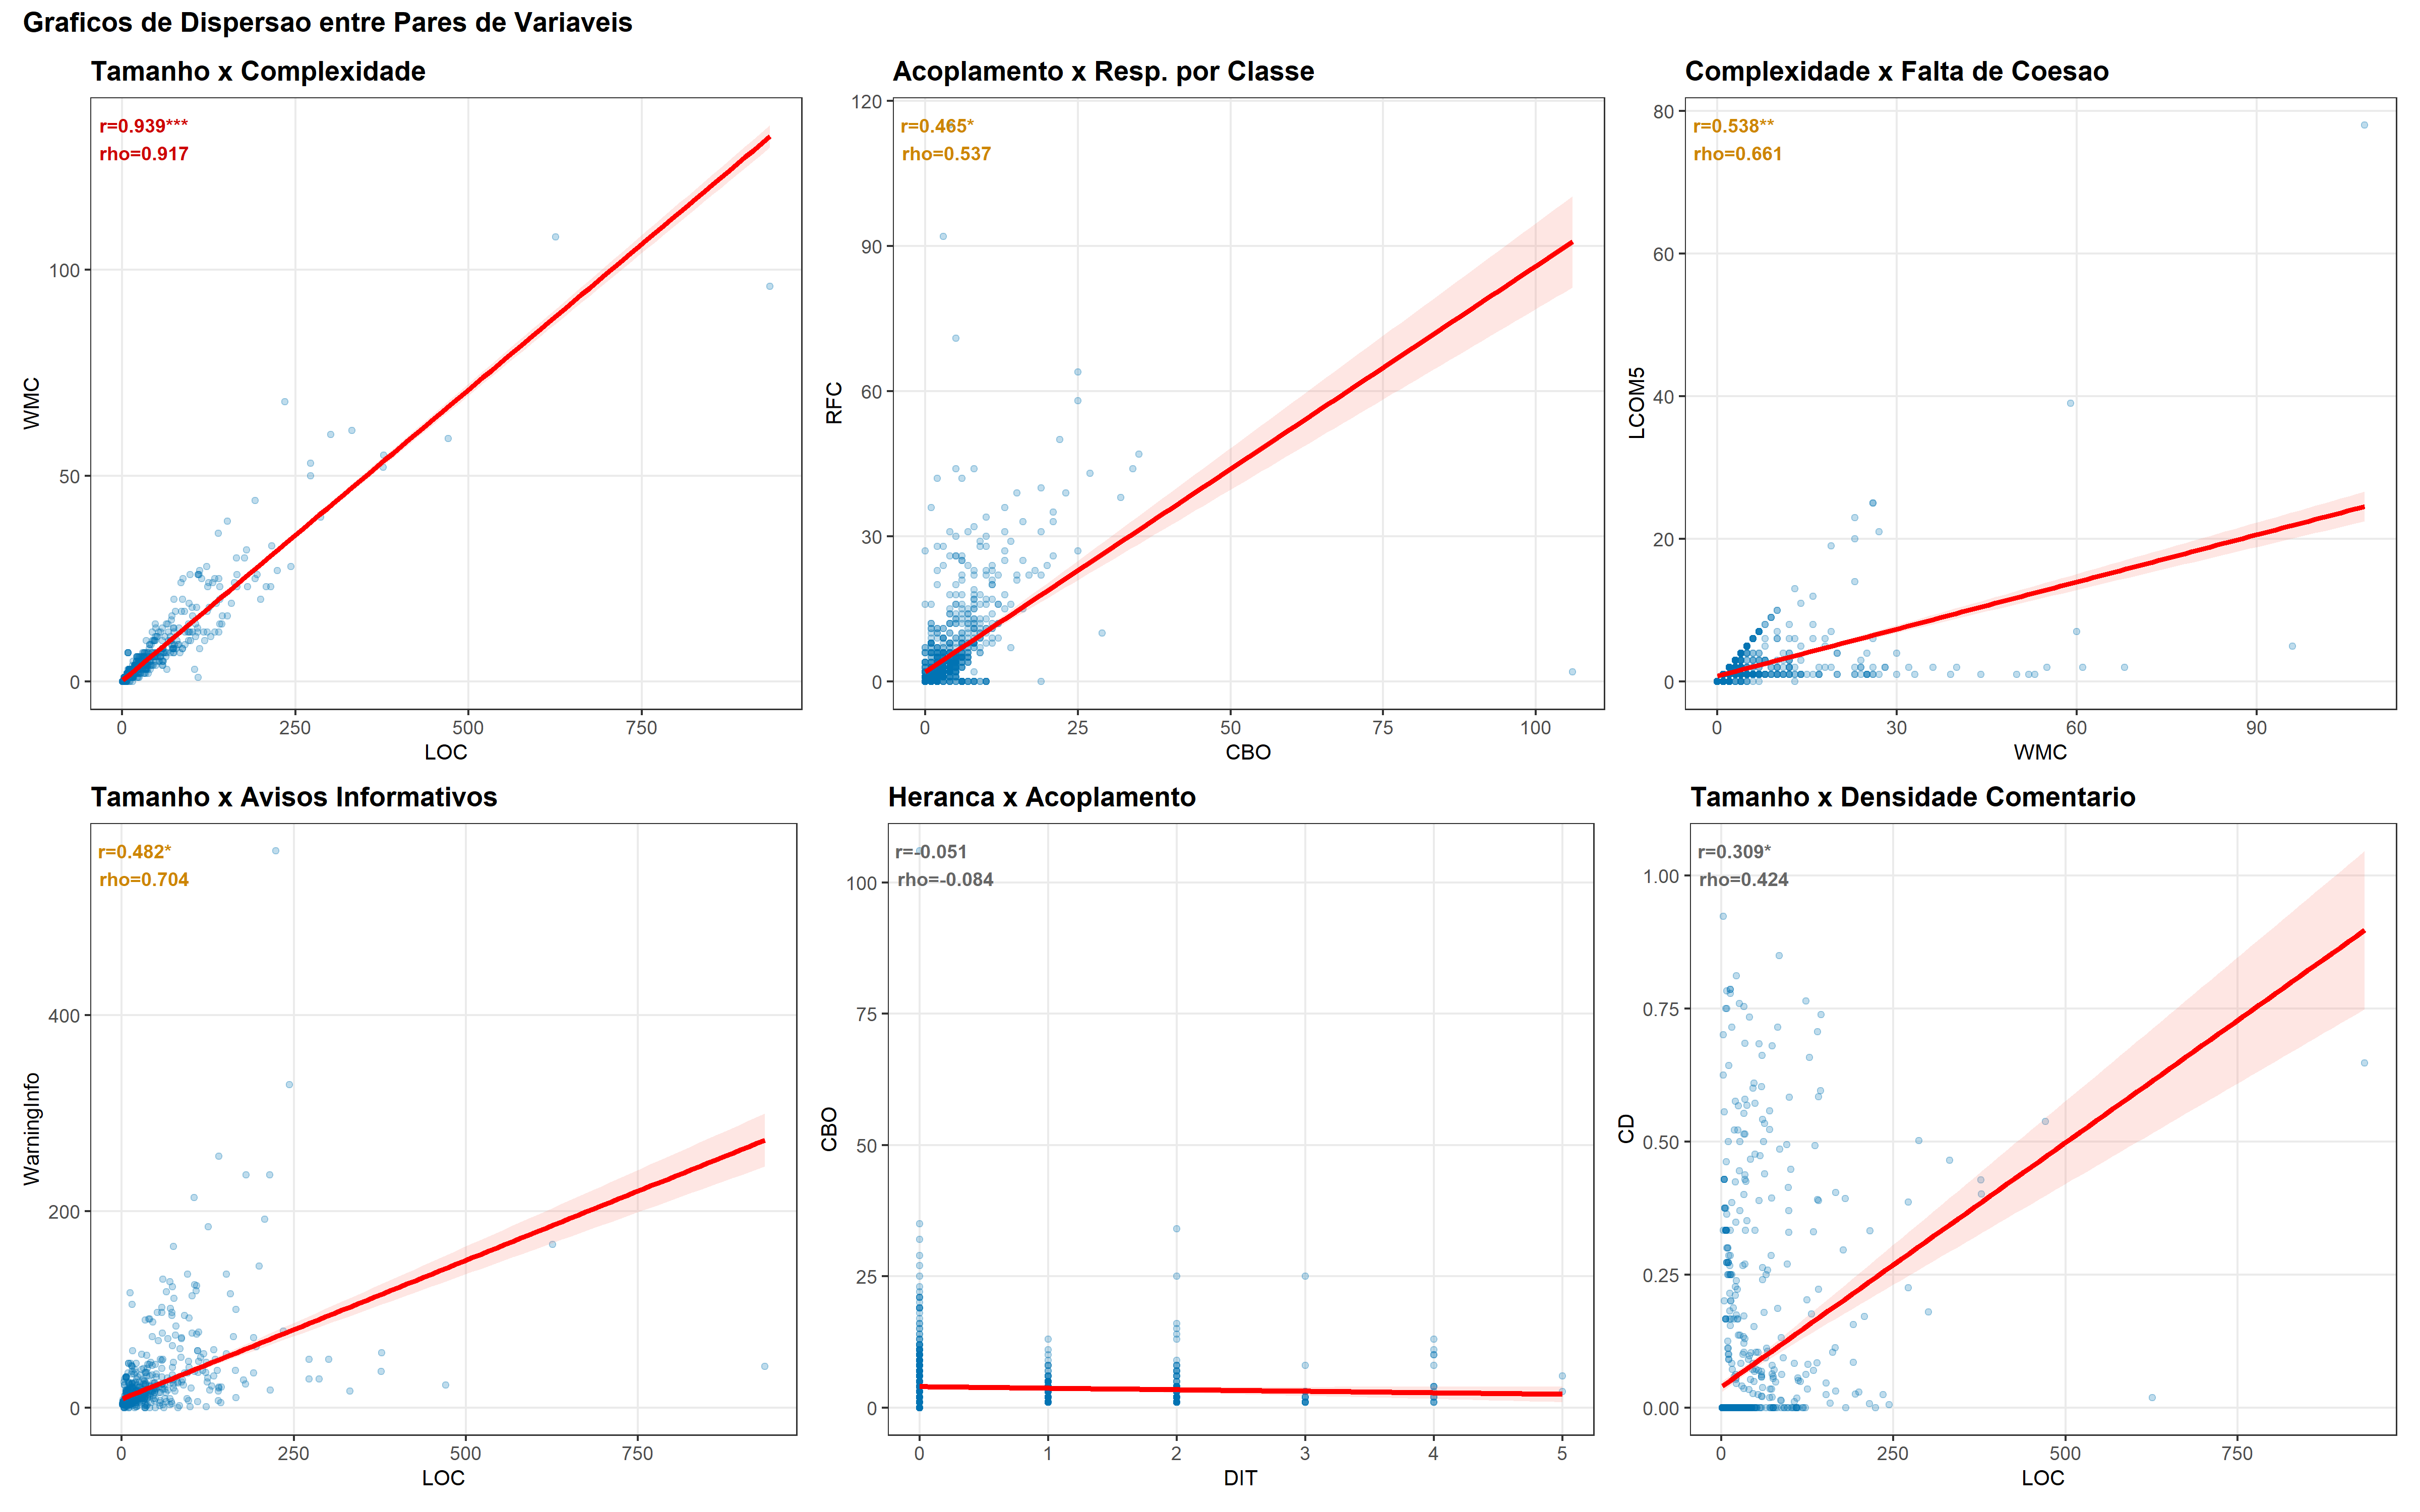
\includegraphics[width=\linewidth]{../output/figures_r/scatter_plots_r.png}
  \caption{Gráficos de dispersão com linha de regressão linear ajustada
           e coeficientes de correlação.}
  \label{fig:scatter}
\end{figure}

\subsubsection{Distribuição de DIT}

A Figura~\ref{fig:dit} apresenta a distribuição de frequências de DIT.
Observa-se que 54\% das classes têm DIT = 0 (sem herança) e apenas 5
classes atingem DIT = 5, confirmando que o JUnit utiliza herança de
forma conservadora.

\begin{figure}[H]
  \centering
  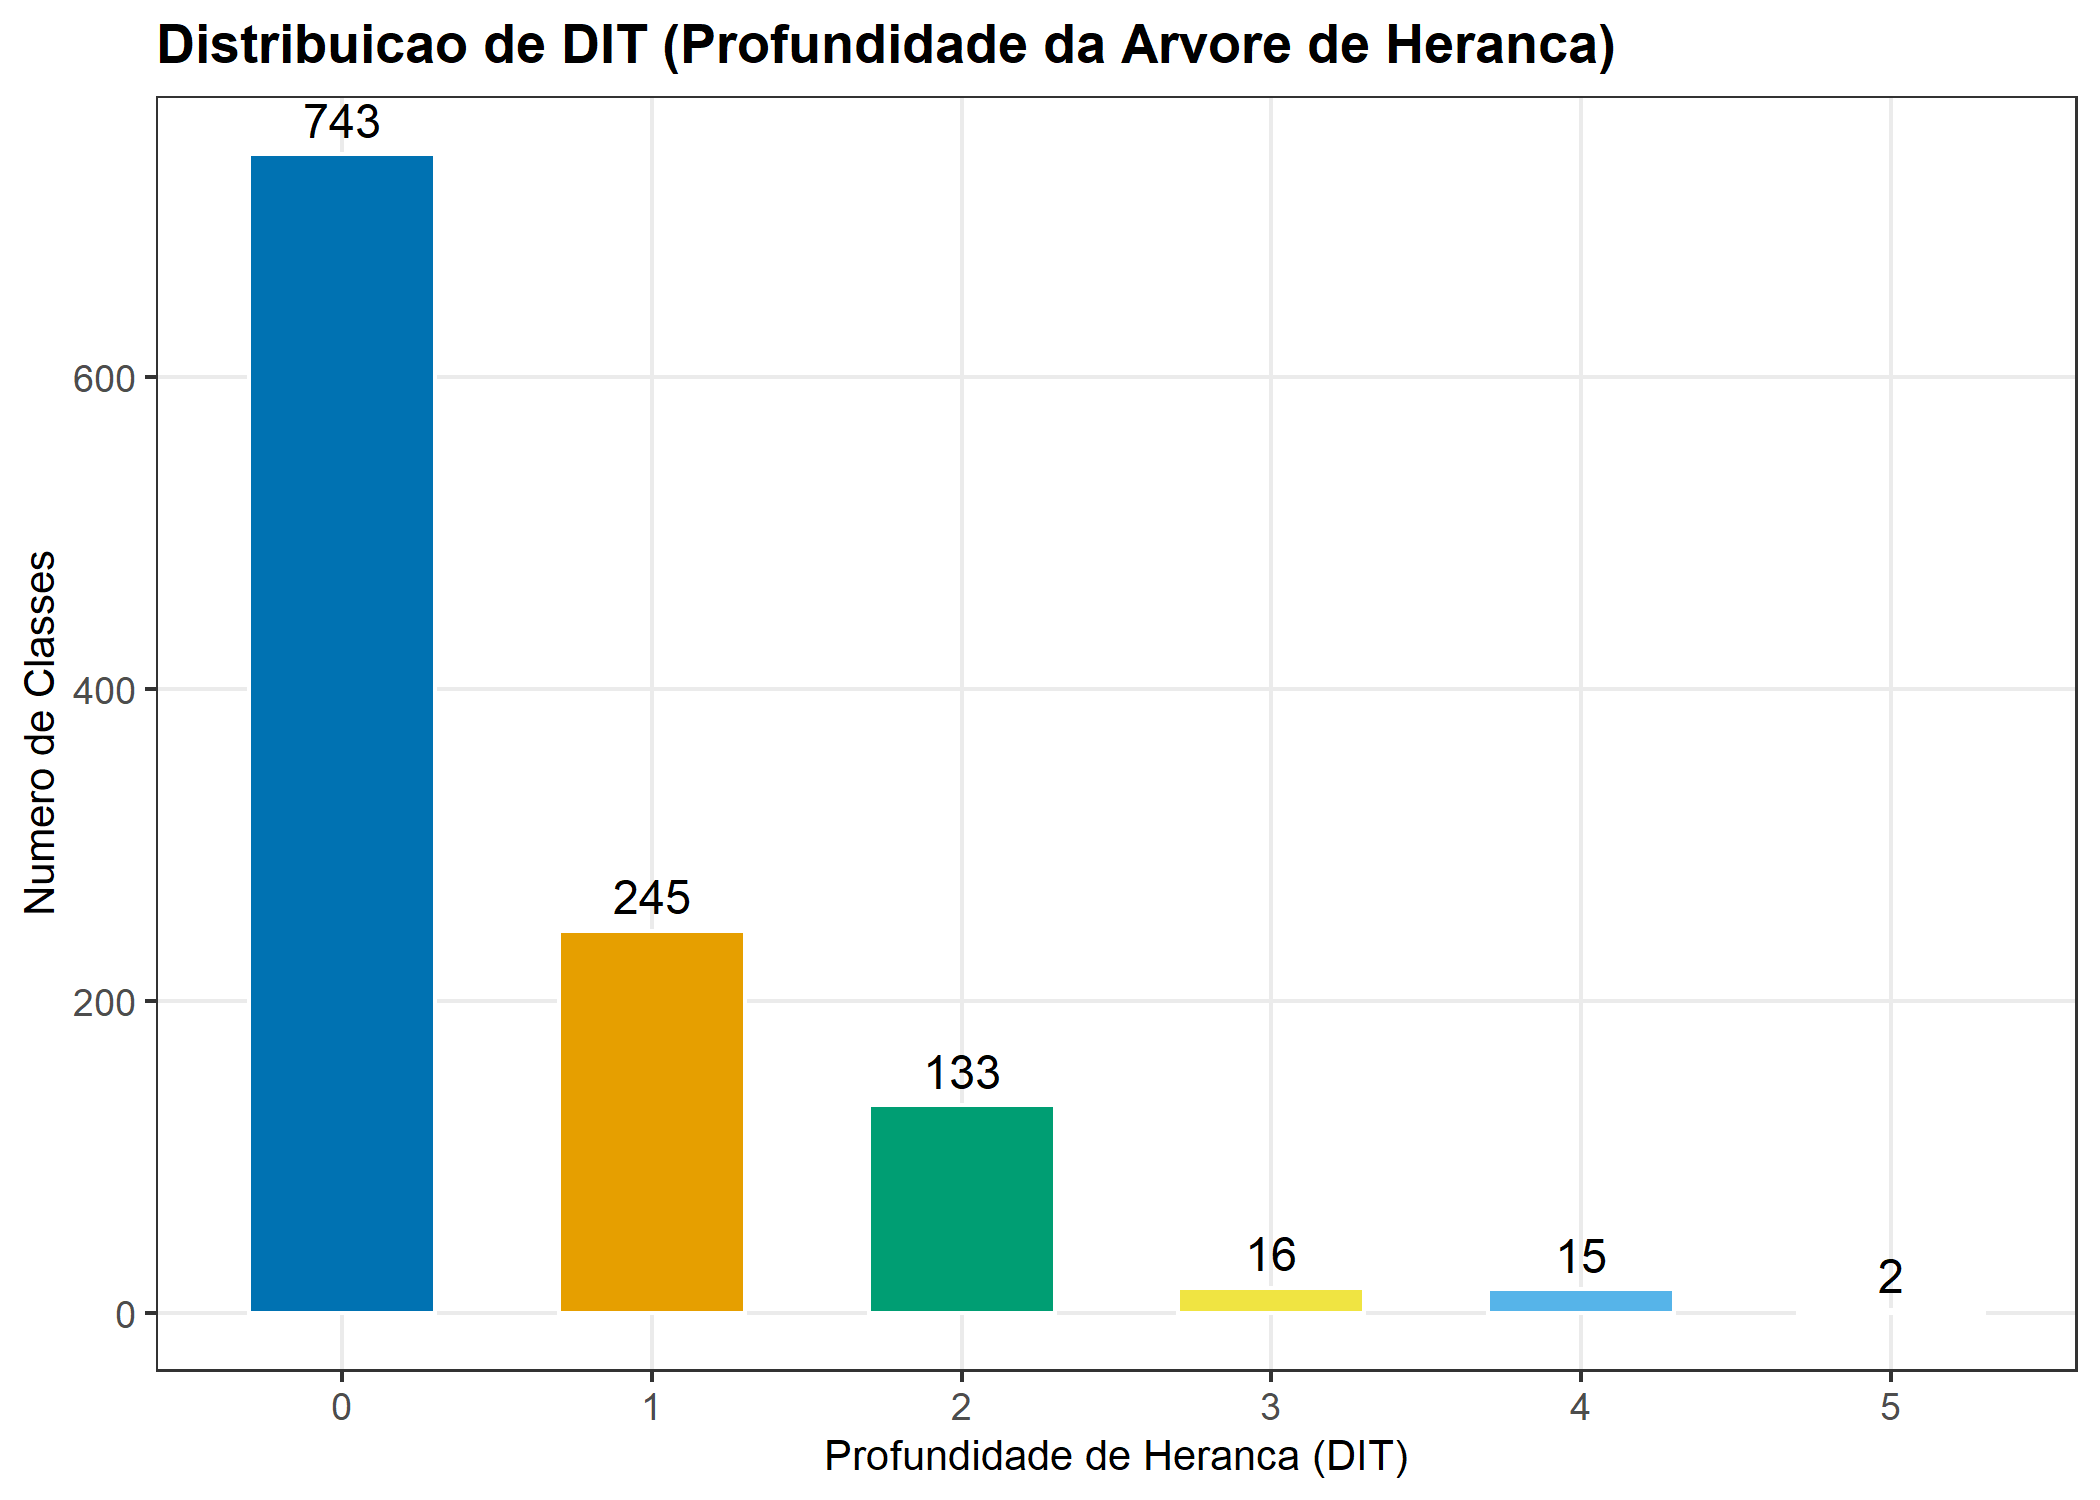
\includegraphics[width=0.55\linewidth]{../output/figures_r/bar_dit_r.png}
  \caption{Distribuição de frequências da profundidade de herança (DIT).}
  \label{fig:dit}
\end{figure}

\subsection{Avaliação de Outliers}
\label{sec:outliers}

A Tabela~\ref{tab:outliers} resume a análise de outliers pelo método
IQR. A Figura~\ref{fig:outlier_boxplots} complementa com os boxplots
anotados.

\begin{table}[H]
\centering
\caption{Contagem de outliers pelo método IQR (limiar $= 1{,}5 \times IQR$)}
\label{tab:outliers}
\begin{tabular}{lrrrrr}
\toprule
\textbf{Variável} & \textbf{Q1} & \textbf{Q3} & \textbf{Fence Sup.} & \textbf{N Outliers} & \textbf{\% Outliers} \\
\midrule
WMC          & 1,0 & 4,00  & 8,5   & 120 & 10,4 \\
CBO          & 1,0 & 5,00  & 11,0  & 42  & 3,6  \\
LCOM5        & 1,0 & 2,00  & 3,5   & 95  & 8,2  \\
DIT          & 0,0 & 1,00  & 2,5   & 33  & 2,9  \\
RFC          & 1,0 & 5,00  & 11,0  & 131 & 11,4 \\
LOC          & 6,0 & 22,75 & 47,9  & 155 & 13,4 \\
NM           & 1,0 & 7,00  & 16,0  & 149 & 12,9 \\
WarningInfo  & 5,0 & 14,00 & 27,5  & 142 & 12,3 \\
WarningMajor & 0,0 & 1,00  & 2,5   & 172 & 14,9 \\
CD           & 0,0 & 0,00  & 0,0   & 253 & 21,9 \\
\bottomrule
\end{tabular}
\end{table}

\begin{figure}[H]
  \centering
  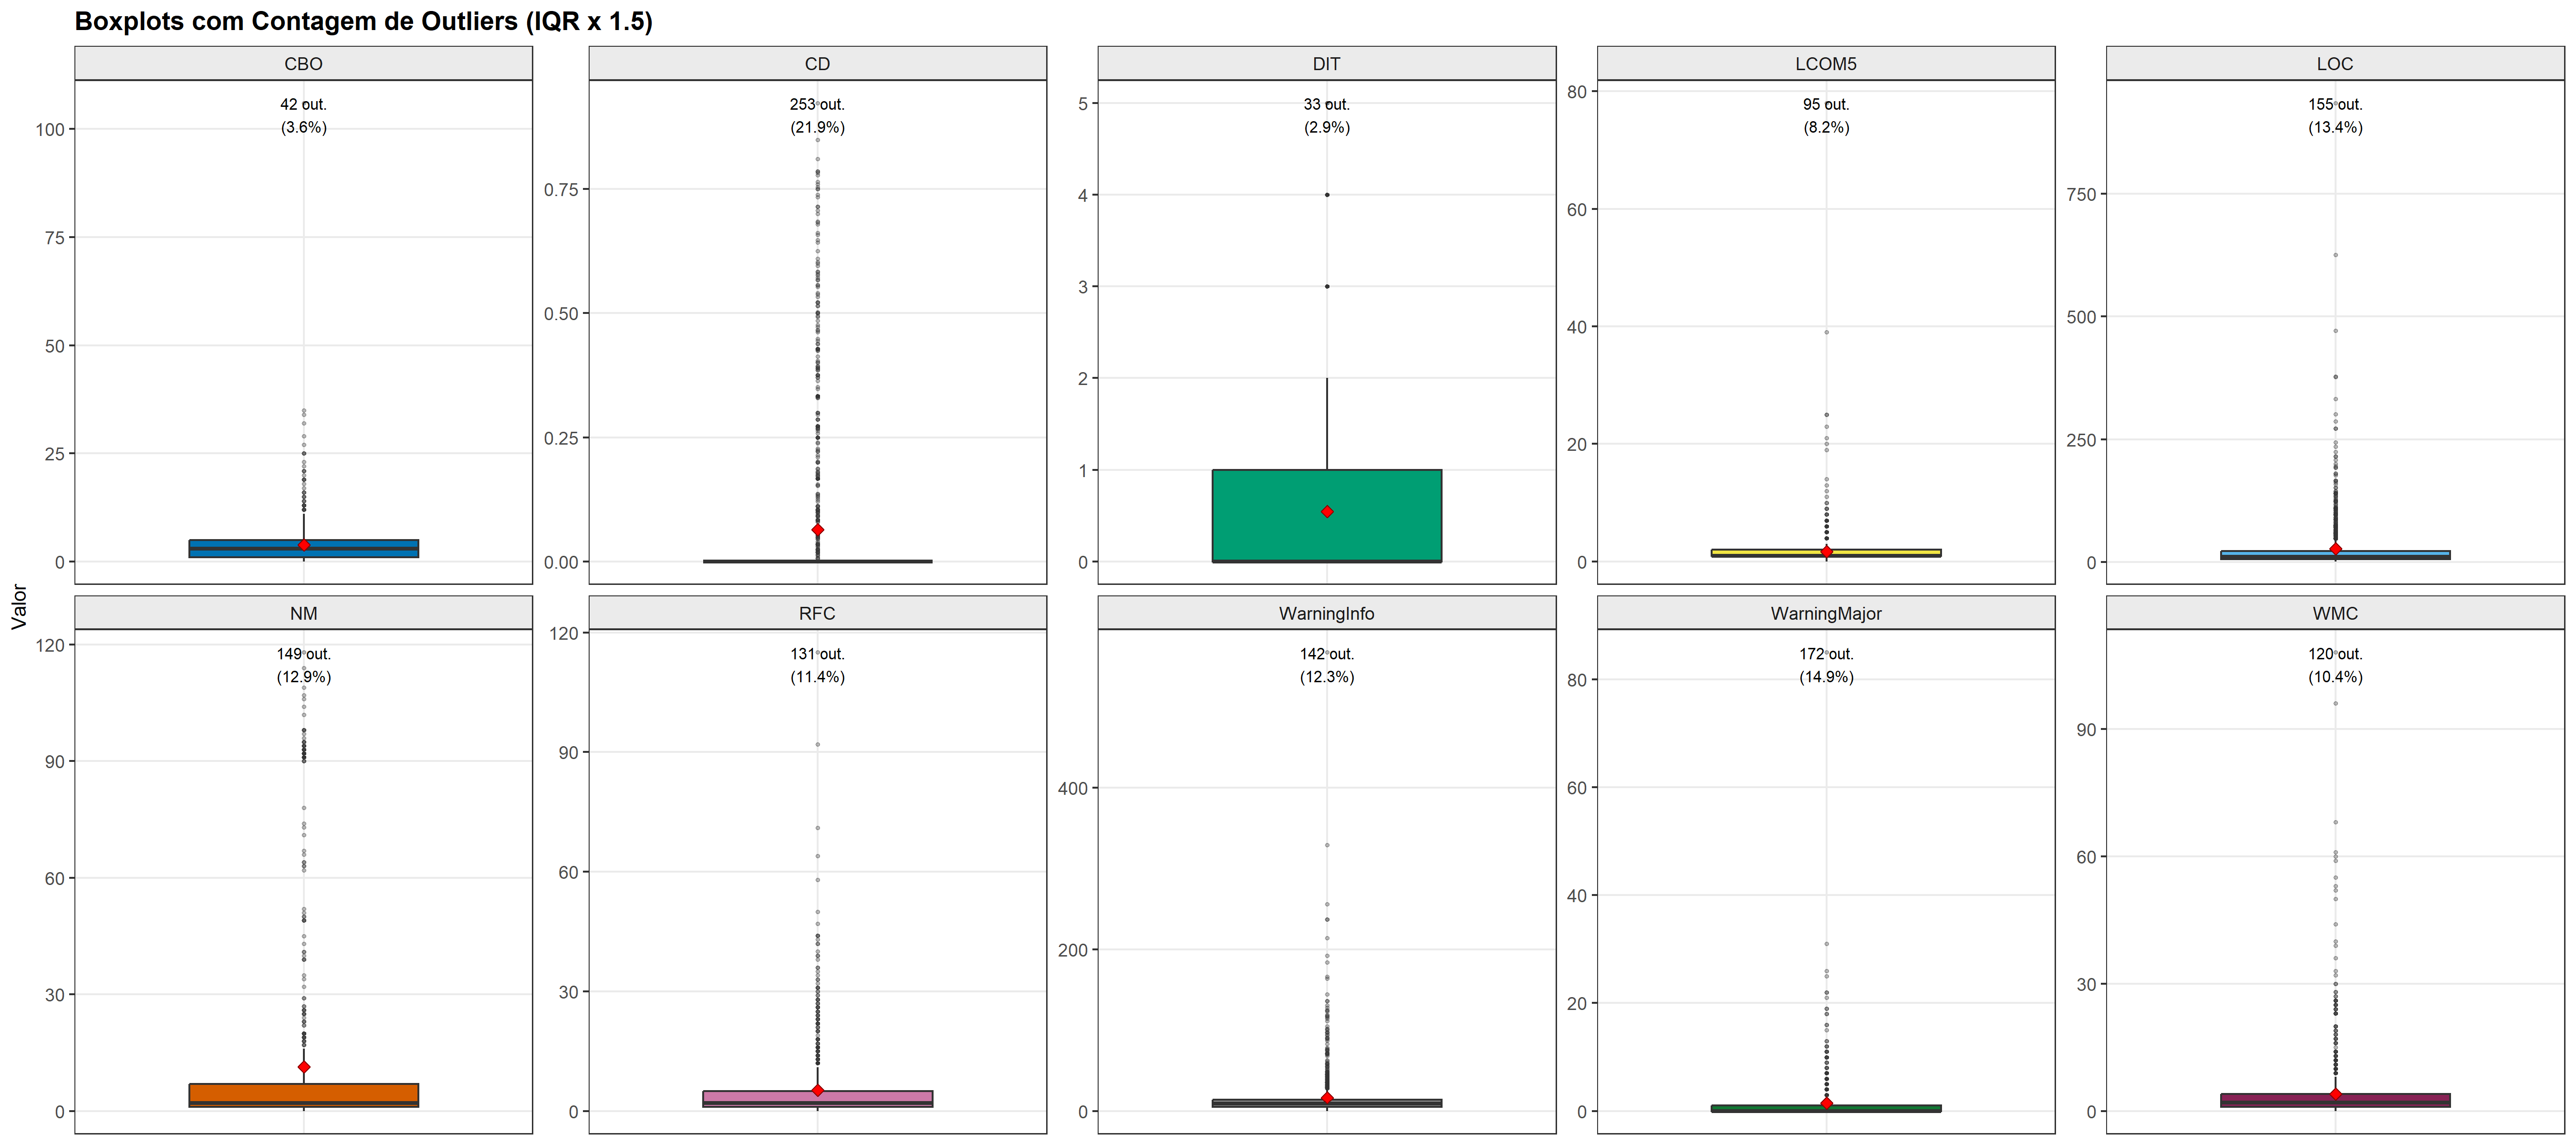
\includegraphics[width=\linewidth]{../output/figures_r/outlier_boxplots_r.png}
  \caption{Boxplots com contagem e percentual de outliers anotados.}
  \label{fig:outlier_boxplots}
\end{figure}

Os outliers de LOC correspondem às chamadas \textit{God Classes} — classes
que concentram responsabilidades excessivas, violando o Princípio da
Responsabilidade Única (SRP). As principais identificadas são:
\texttt{Assert} (935 LOC, WMC=96), \texttt{AssertionTest} (626 LOC, WMC=108)
e \texttt{TestCase} (471 LOC, WMC=59).

\subsection{Testes de Normalidade}
\label{sec:normalidade}

A Tabela~\ref{tab:normalidade} apresenta os resultados dos testes de
Shapiro-Wilk (SW) e Kolmogorov-Smirnov com correção de Lilliefors (KS).
A Figura~\ref{fig:qqplots} exibe os Q-Q plots.

\begin{table}[H]
\centering
\caption{Testes de normalidade (Shapiro-Wilk e Kolmogorov-Smirnov)}
\label{tab:normalidade}
\begin{tabular}{lrrrrl}
\toprule
\textbf{Variável} & \textbf{SW W} & \textbf{SW p} & \textbf{KS D} & \textbf{KS p} & \textbf{Normal?} \\
\midrule
WMC          & 0,4297 & $<$0,001 & 0,3085 & $<$0,001 & Não \\
CBO          & 0,5097 & $<$0,001 & 0,2333 & $<$0,001 & Não \\
LCOM5        & 0,3015 & $<$0,001 & 0,3255 & $<$0,001 & Não \\
DIT          & 0,6657 & $<$0,001 & 0,3789 & $<$0,001 & Não \\
RFC          & 0,5295 & $<$0,001 & 0,2759 & $<$0,001 & Não \\
LOC          & 0,4076 & $<$0,001 & 0,3170 & $<$0,001 & Não \\
NM           & 0,4688 & $<$0,001 & 0,3499 & $<$0,001 & Não \\
WarningInfo  & 0,3853 & $<$0,001 & 0,3080 & $<$0,001 & Não \\
WarningMajor & 0,3526 & $<$0,001 & 0,3534 & $<$0,001 & Não \\
CD           & 0,4664 & $<$0,001 & 0,4360 & $<$0,001 & Não \\
\bottomrule
\end{tabular}
\end{table}

\begin{figure}[H]
  \centering
  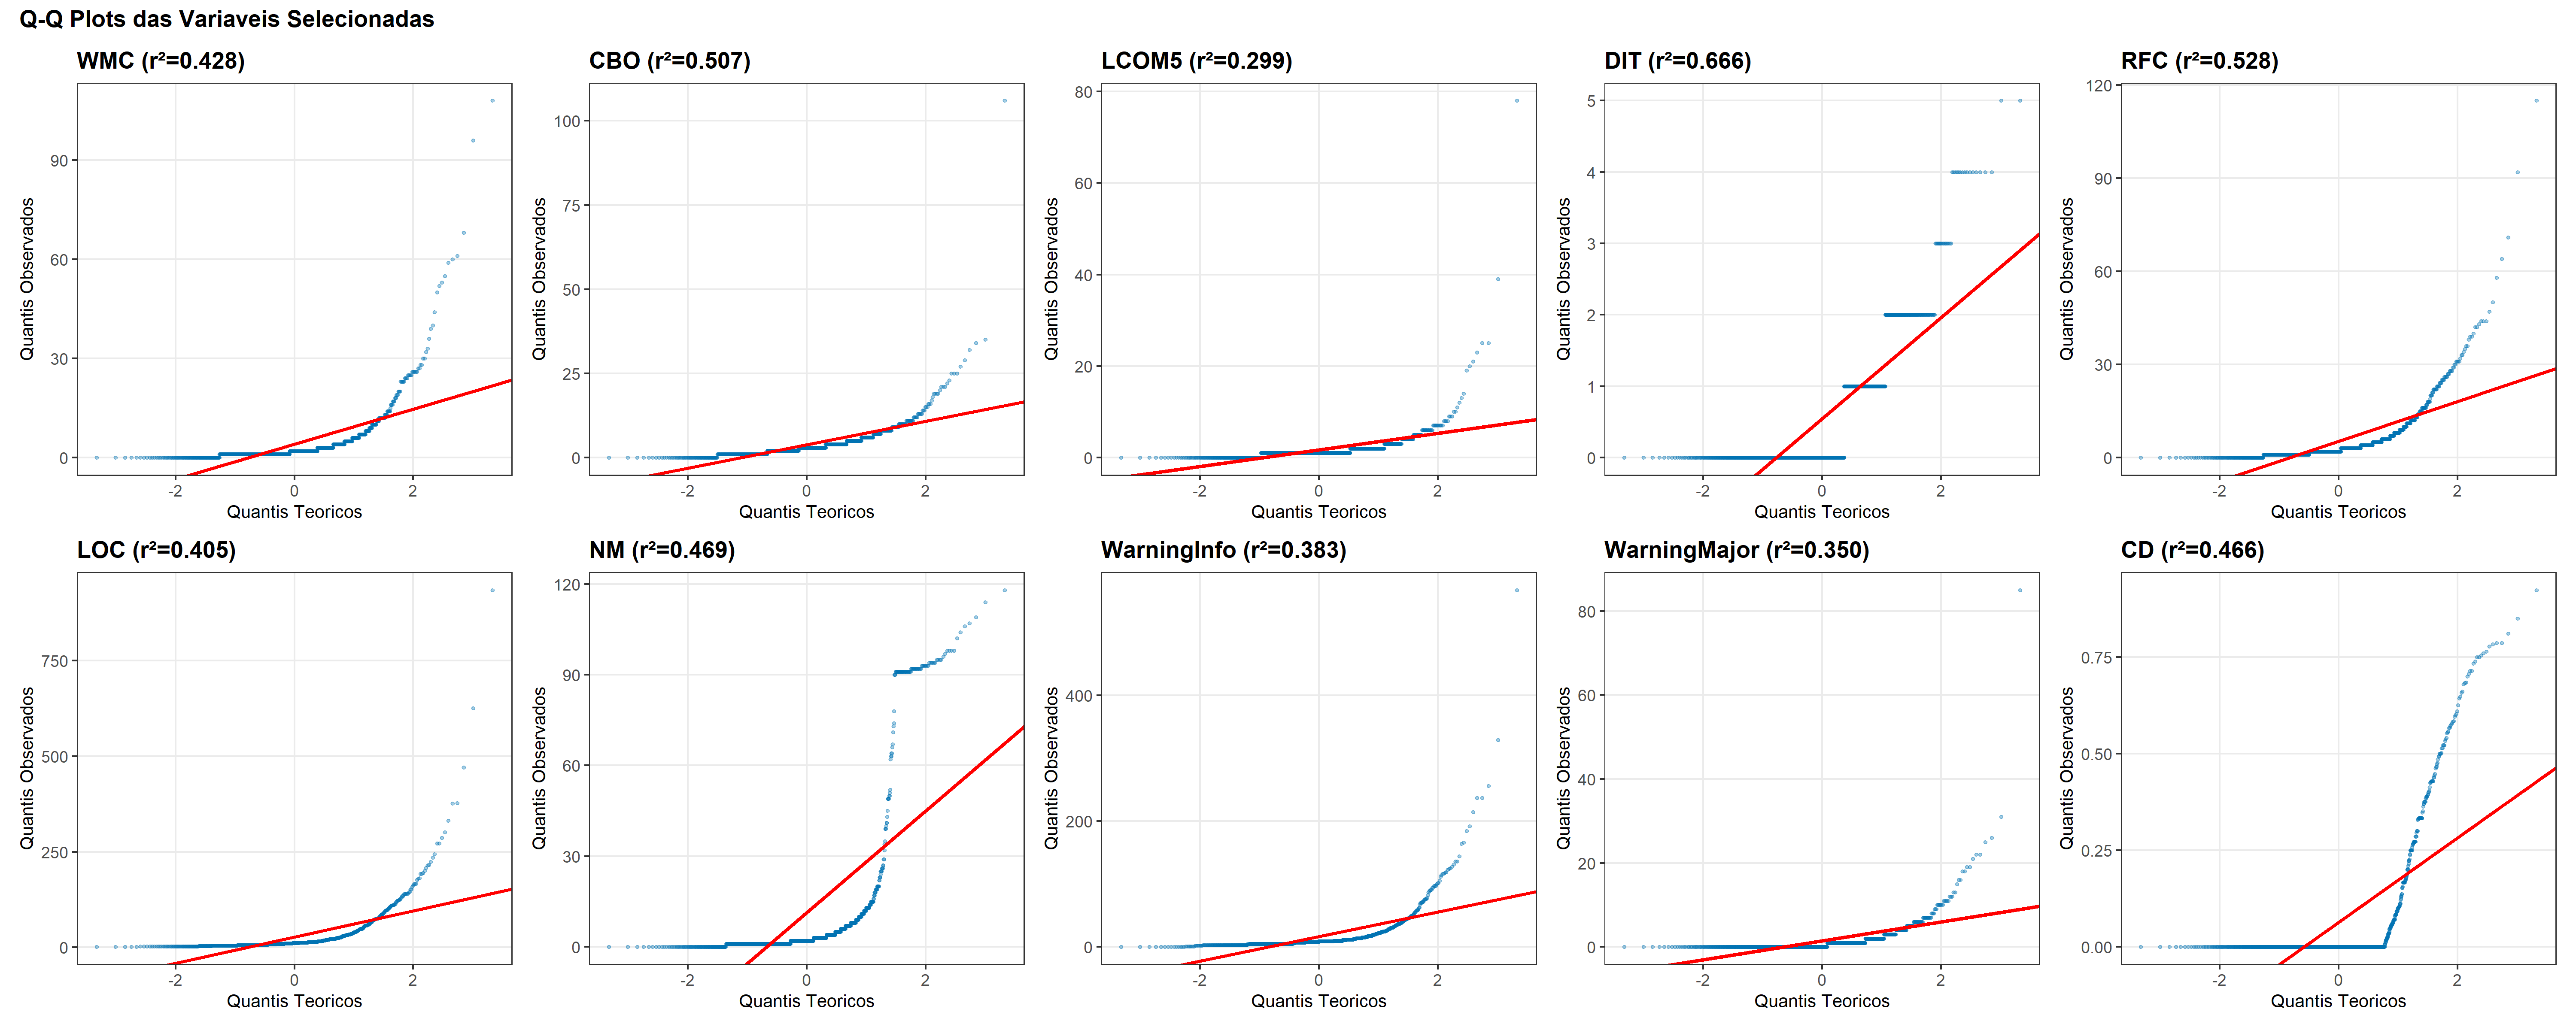
\includegraphics[width=\linewidth]{../output/figures_r/qq_plots_r.png}
  \caption{Q-Q plots das variáveis selecionadas. Desvios sistemáticos
           da linha vermelha indicam não-normalidade.}
  \label{fig:qqplots}
\end{figure}

Todos os 20 testes aplicados rejeitam a hipótese de normalidade com
$p < 0{,}001$. Os Q-Q plots confirmam a cauda pesada à direita em todas
as variáveis. Mesmo após a transformação $\log(1+x)$, nenhuma variável
atinge normalidade, embora os p-valores melhorem substancialmente
(e.g., WMC: $p = 4{,}7 \times 10^{-51} \to 3{,}1 \times 10^{-28}$).

\subsection{Análise de Correlação}
\label{sec:correlacao}

A Figura~\ref{fig:heatmap} apresenta o mapa de calor das correlações de
Pearson entre as dez variáveis.

\begin{figure}[H]
  \centering
  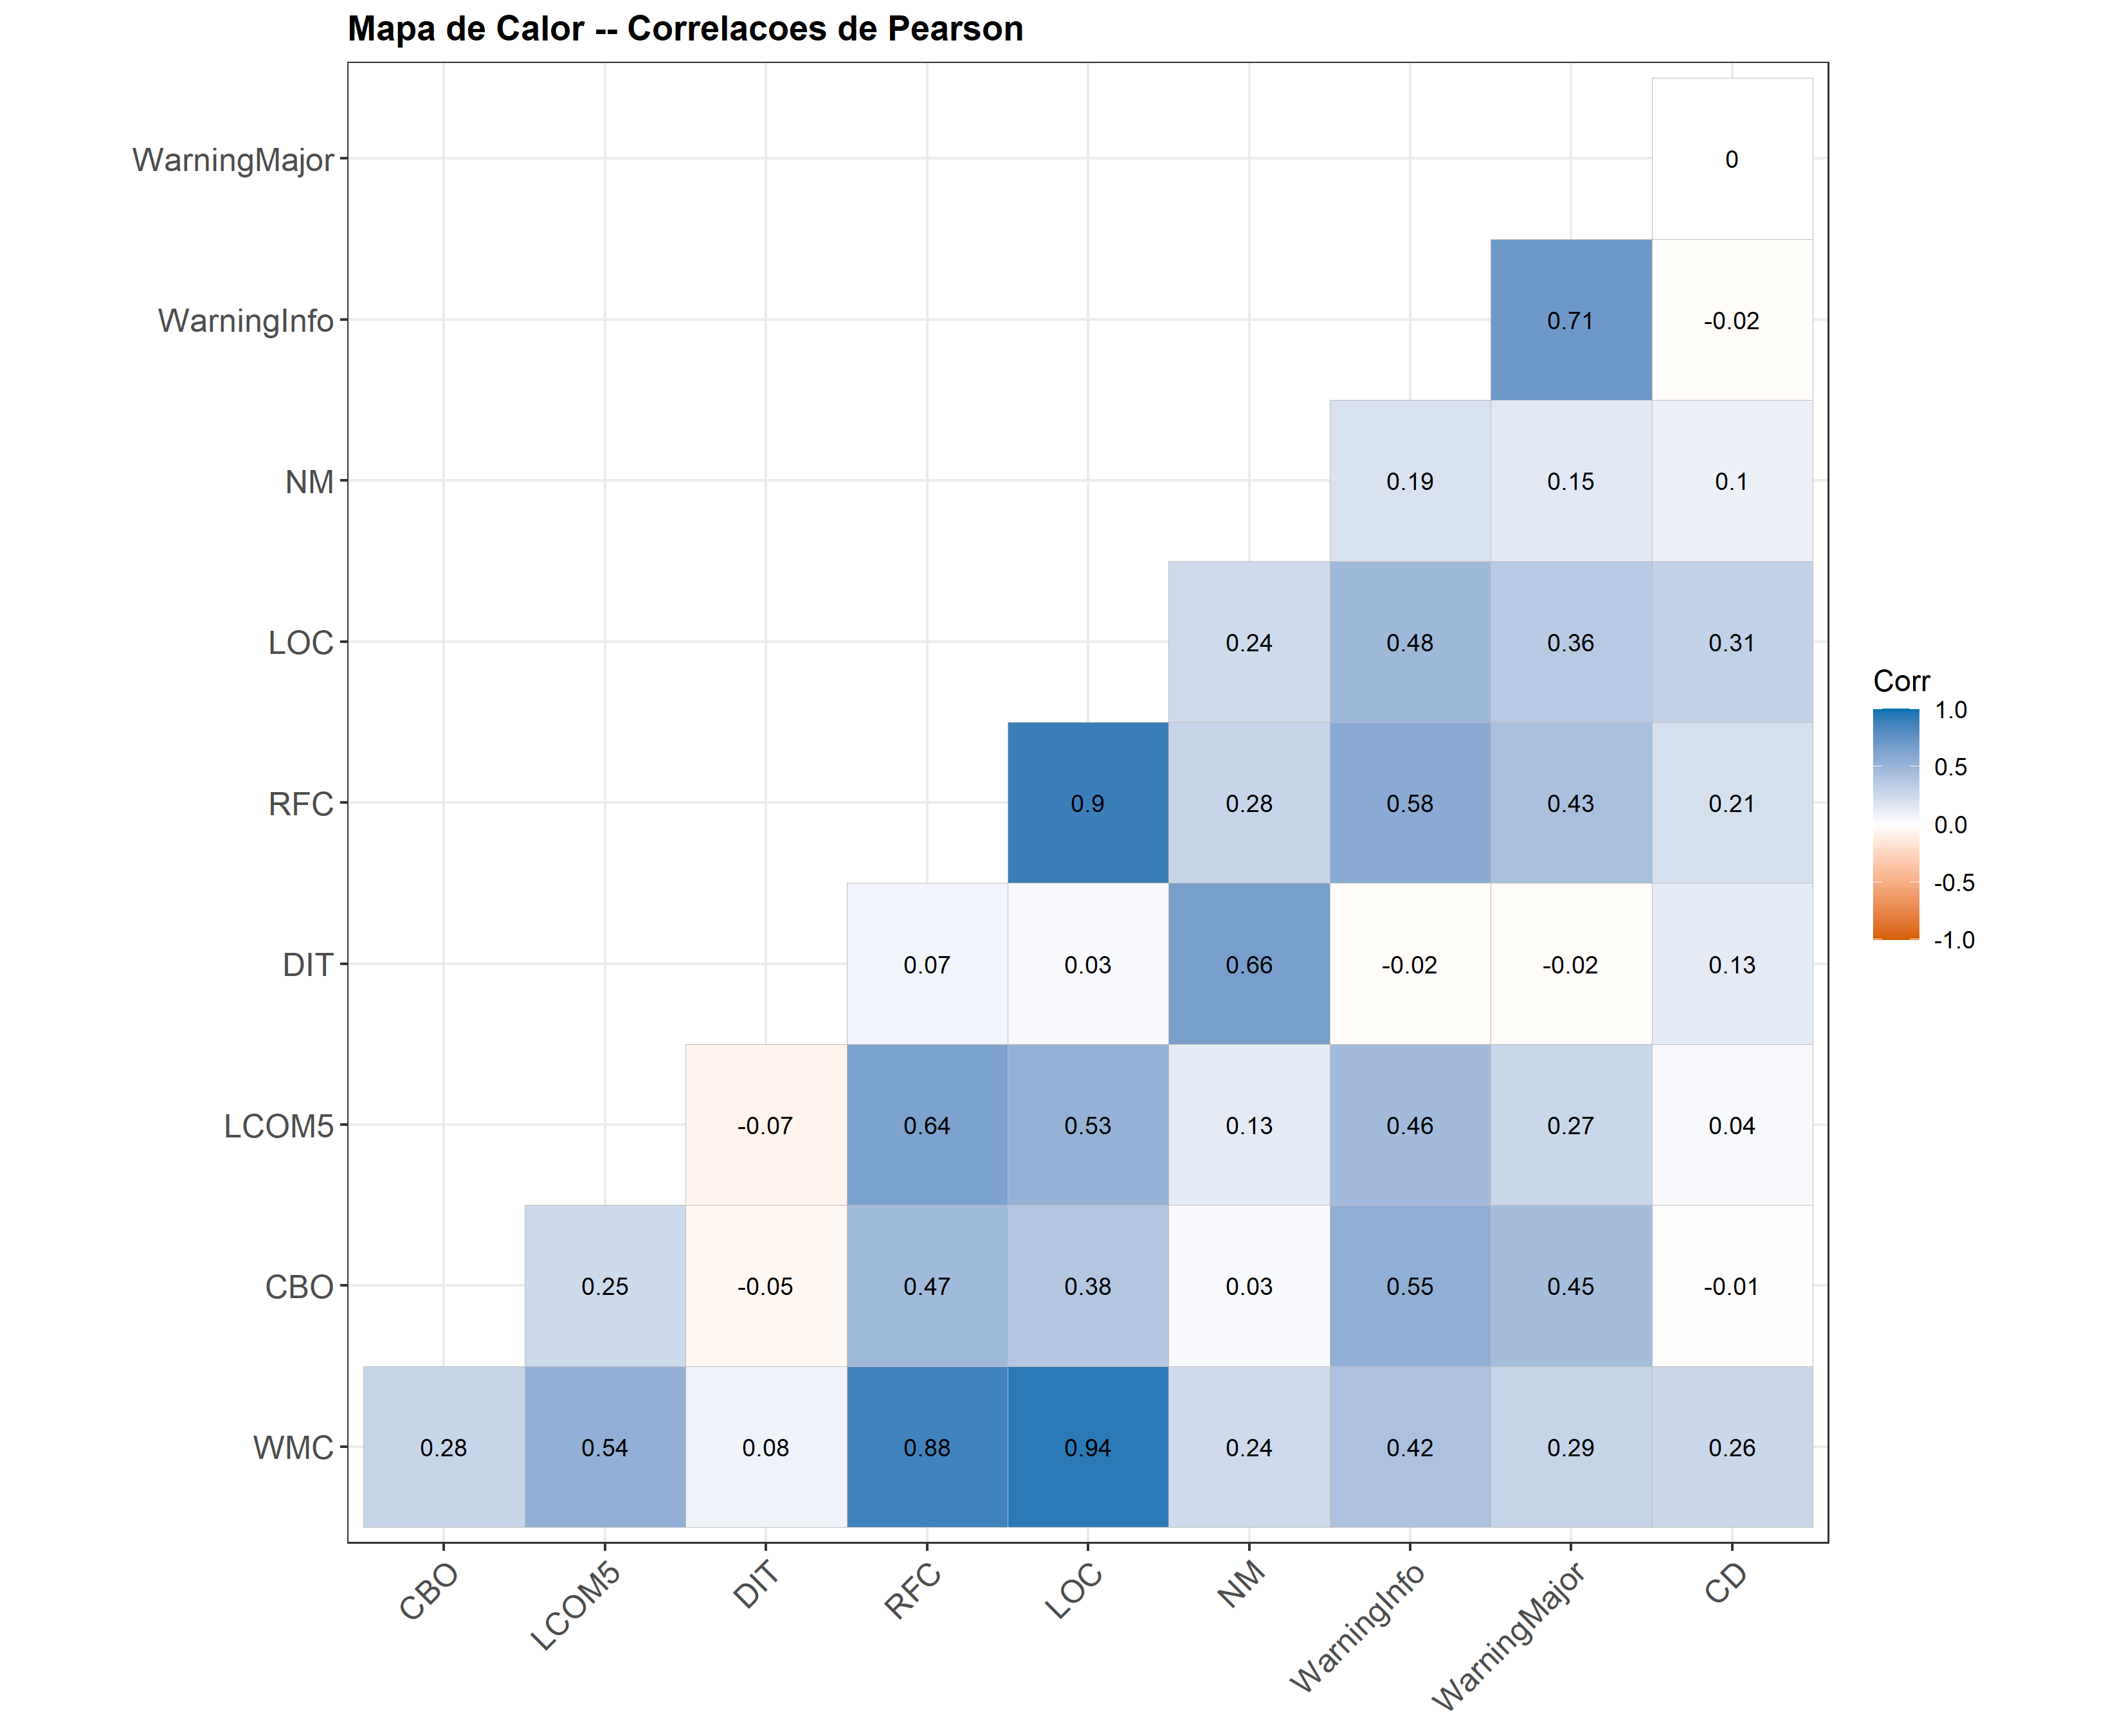
\includegraphics[width=0.85\linewidth]{../output/figures_r/correlation_heatmap_r.png}
  \caption{Mapa de calor das correlações de Pearson. Azul indica correlação
           positiva; vermelho indica correlação negativa.}
  \label{fig:heatmap}
\end{figure}

A Figura~\ref{fig:pairgrid} apresenta a matriz completa no estilo da
função \texttt{chart.Correlation()} do pacote \texttt{PerformanceAnalytics},
incluindo histogramas na diagonal, gráficos de dispersão no triângulo
inferior e coeficientes de correlação no triângulo superior.

\begin{figure}[H]
  \centering
  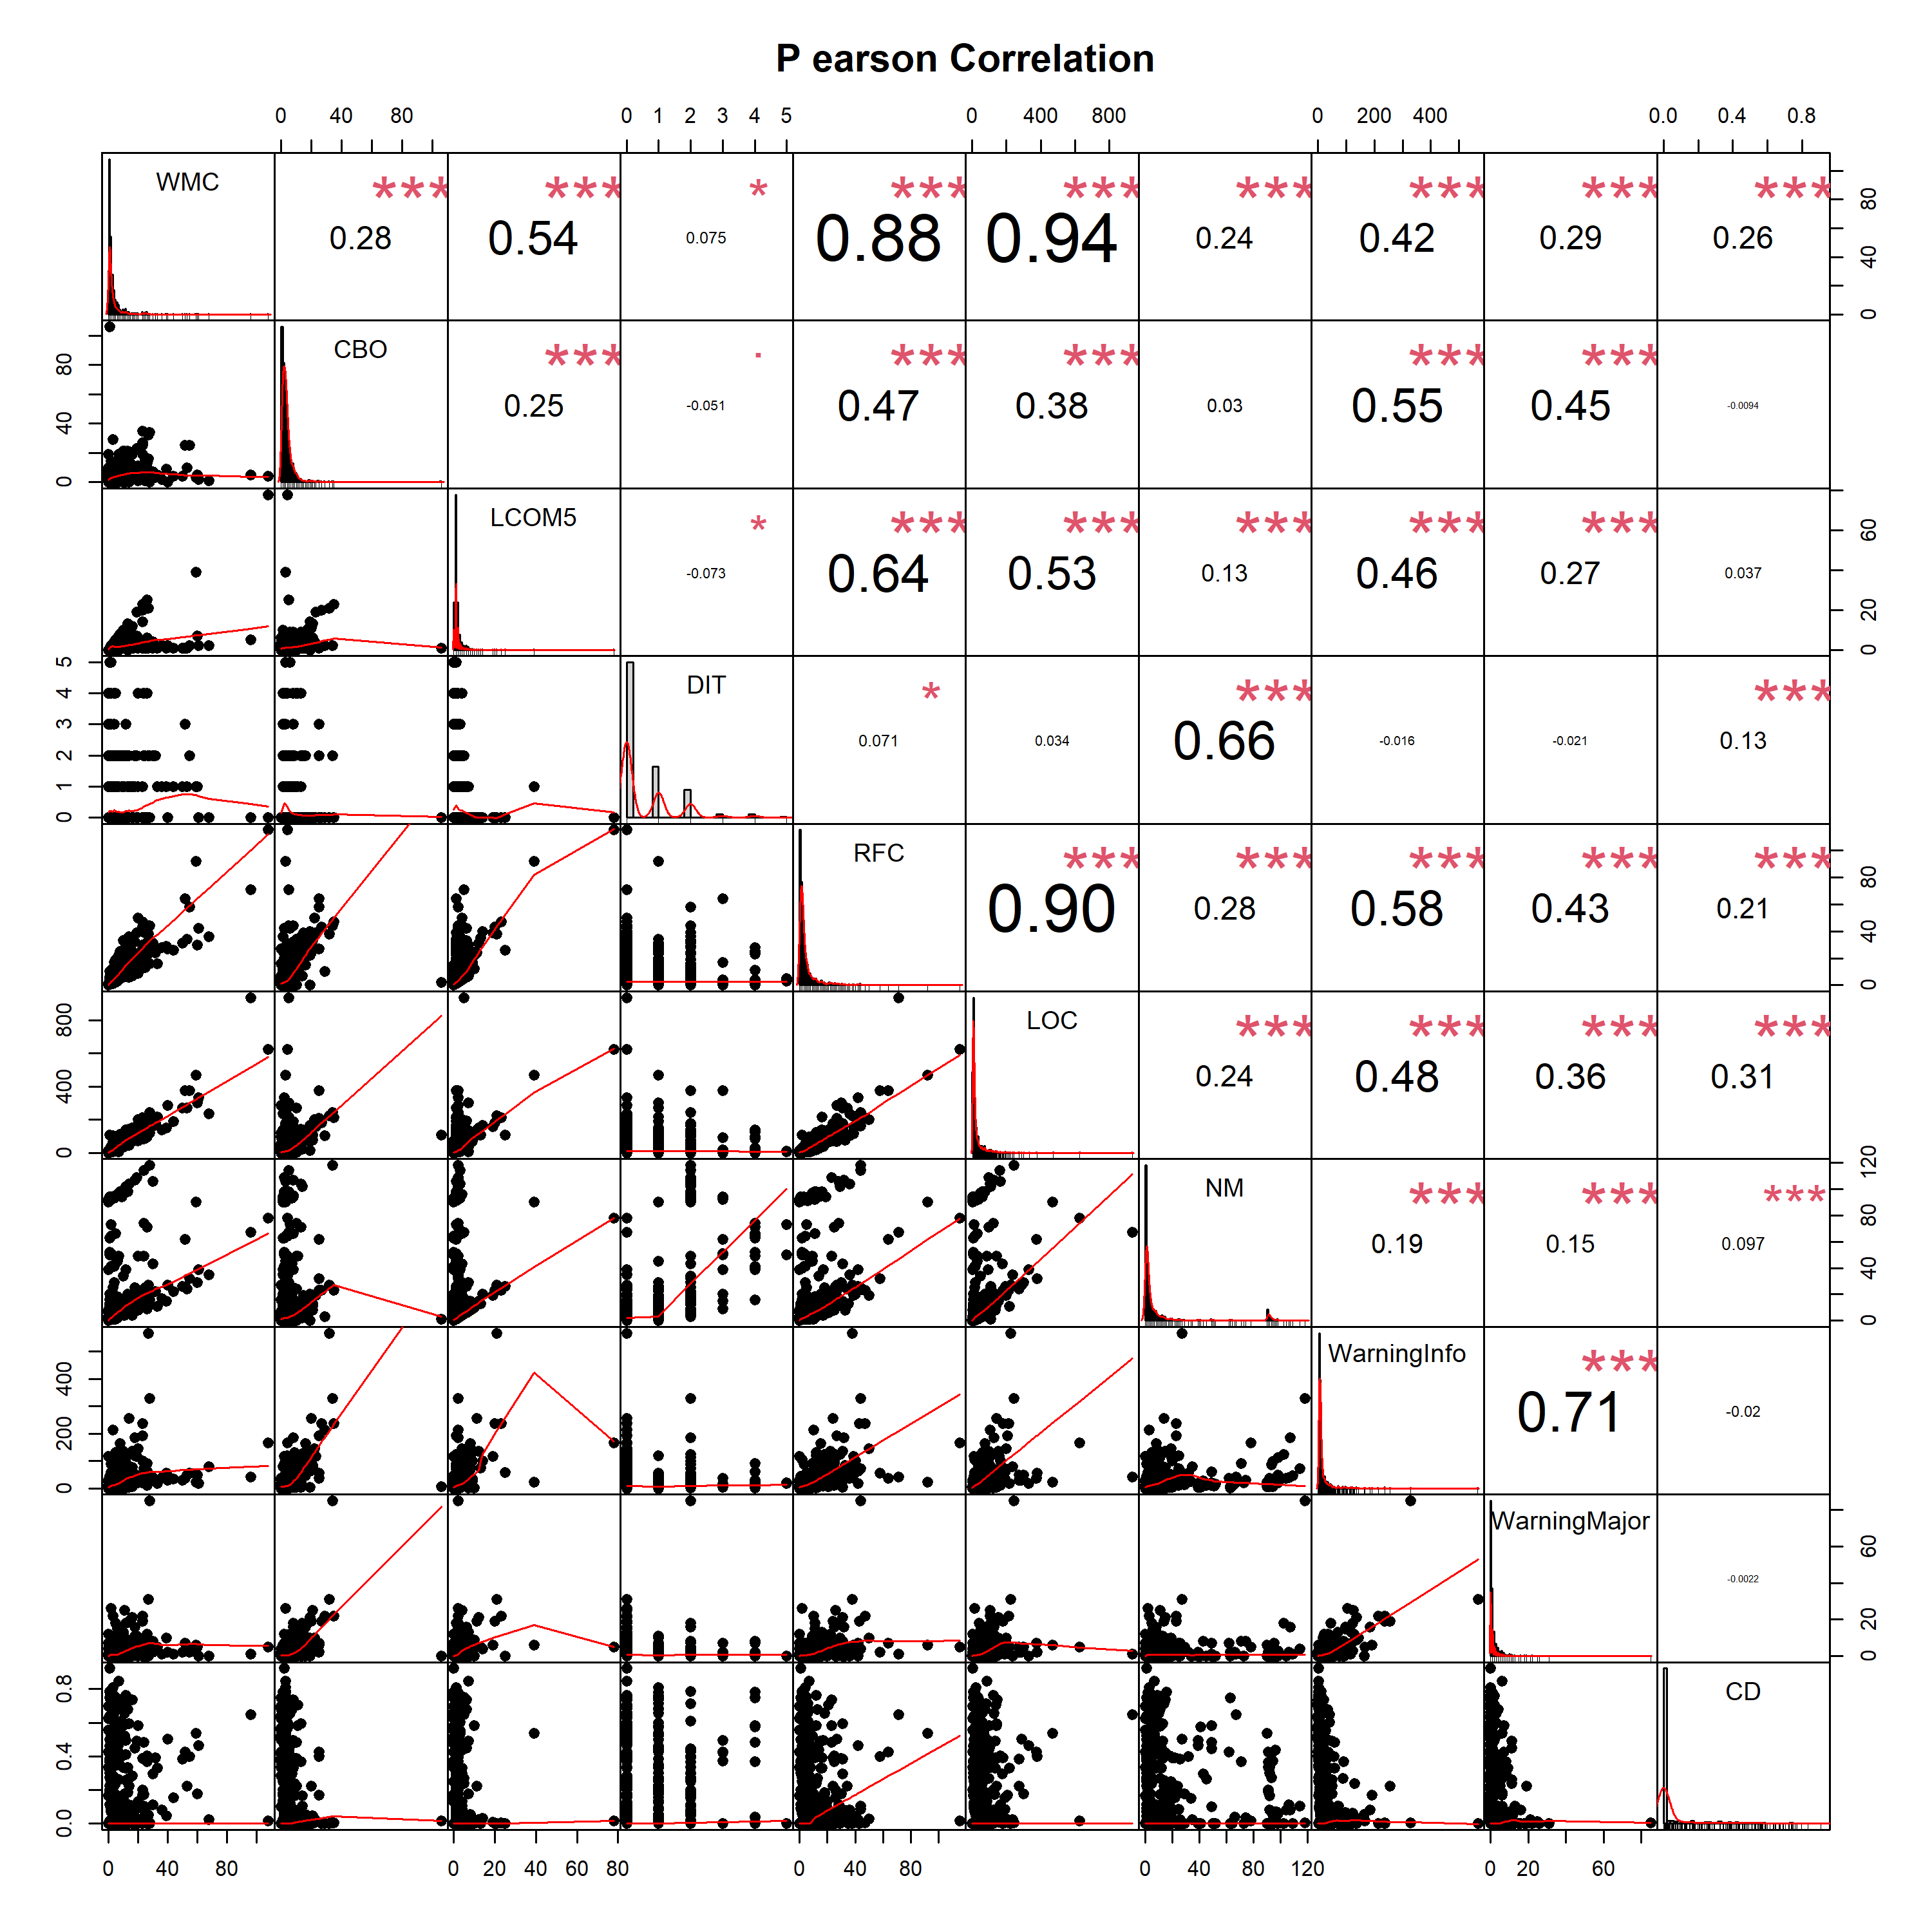
\includegraphics[width=\linewidth]{../output/figures_r/chart_correlation_r.png}
  \caption{Matriz de correlação com histogramas, gráficos de dispersão e
           coeficientes de Pearson (*** $p<0{,}001$, ** $p<0{,}01$, * $p<0{,}05$).}
  \label{fig:pairgrid}
\end{figure}

As principais correlações identificadas são apresentadas na
Tabela~\ref{tab:correlacoes}.

\begin{table}[H]
\centering
\caption{Principais pares de correlação (Pearson)}
\label{tab:correlacoes}
\begin{tabular}{llll}
\toprule
\textbf{Par} & \textbf{r (Pearson)} & \textbf{$\rho$ (Spearman)} & \textbf{Intensidade} \\
\midrule
LOC $\times$ WMC          & 0,939 & 0,917 & Forte   \\
LOC $\times$ RFC          & 0,898 & 0,901 & Forte   \\
WMC $\times$ RFC          & 0,881 & 0,888 & Forte   \\
WarningInfo $\times$ WarningMajor & 0,707 & 0,424 & Forte \\
LCOM5 $\times$ RFC        & 0,643 & 0,603 & Moderada \\
DIT $\times$ NM           & 0,655 & 0,526 & Moderada \\
LCOM5 $\times$ WMC        & 0,538 & 0,661 & Moderada \\
CBO $\times$ RFC          & 0,465 & 0,537 & Moderada \\
LOC $\times$ WarningInfo  & 0,482 & 0,704 & Moderada \\
DIT $\times$ CBO          & $-0,051$ & $-0,084$ & Fraca \\
DIT $\times$ WMC          & 0,075 & 0,065 & Fraca   \\
\bottomrule
\end{tabular}
\end{table}

\subsection{Modelagem Estatística}
\label{sec:modelagem}

\subsubsection{Regressão Linear Múltipla}

Devido à variância zero da variável ``\textit{Number of bugs}'', adotamos
WMC (complexidade) como variável resposta. Os preditores foram CBO, DIT, NM
e LCOM5 — excluindo LOC para evitar multicolinearidade ($r = 0{,}94$
com WMC).

A Tabela~\ref{tab:regressao_linear} apresenta os coeficientes estimados.
O modelo apresenta $R^2 = 0{,}342$ e $R^2_{adj} = 0{,}340$, com
$F(4,1149) = 149{,}2$ ($p < 0{,}001$), confirmando a significância
global. O VIF máximo entre os preditores é 1,86 (ausência de
multicolinearidade).

\begin{table}[H]
\centering
\caption{Regressão Linear: WMC $\sim$ CBO + DIT + NM + LCOM5}
\label{tab:regressao_linear}
\begin{tabular}{lrrrrl}
\toprule
\textbf{Preditor} & \textbf{Coef.} & \textbf{Erro Pad.} & \textbf{t} & \textbf{p-valor} & \textbf{VIF} \\
\midrule
Intercepto & 0,465 & 0,287 &  1,62 & 0,105 & -- \\
CBO        & 0,248 & 0,041 &  6,04 & $<$0,001 & 1,07 \\
DIT        & 0,018 & 0,303 &  0,06 & 0,953 & 1,84 \\
NM         & 0,058 & 0,011 &  5,41 & $<$0,001 & 1,86 \\
LCOM5      & 1,171 & 0,062 & 18,82 & $<$0,001 & 1,13 \\
\bottomrule
\multicolumn{6}{l}{$R^2 = 0{,}342$; $R^2_{adj} = 0{,}340$; RMSE $= 6{,}56$; MAE $= 3{,}00$}
\end{tabular}
\end{table}

A Figura~\ref{fig:reg_diag} exibe os diagnósticos do modelo.

\begin{figure}[H]
  \centering
  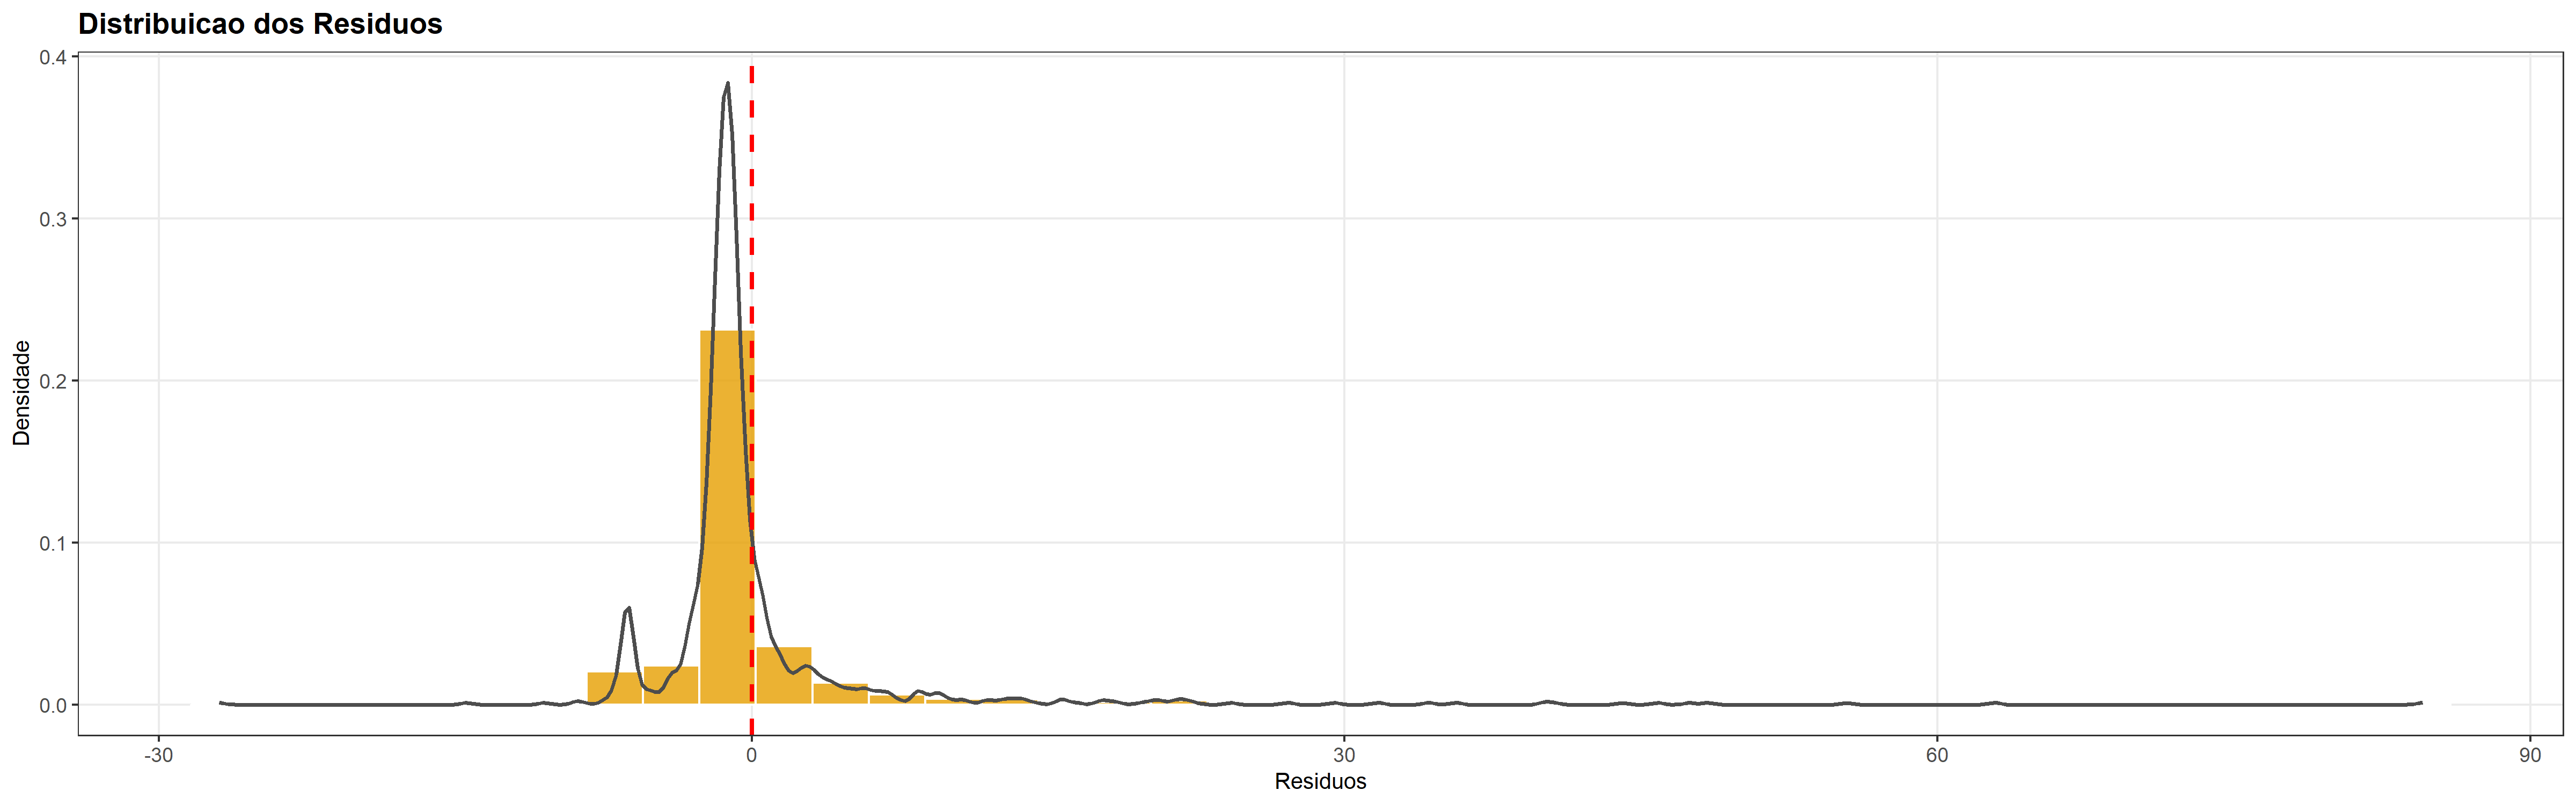
\includegraphics[width=\linewidth]{../output/figures_r/regression_diagnostics_r.png}
  \caption{Diagnósticos da regressão linear: resíduos vs. ajustados (esq.),
           Q-Q dos resíduos (centro) e histograma dos resíduos (dir.).}
  \label{fig:reg_diag}
\end{figure}

O gráfico de resíduos vs. ajustados revela heterocedasticidade (variância
crescente), padrão esperado dado o alto CV das métricas de software.
O Q-Q plot dos resíduos indica cauda pesada à direita, sugerindo que uma
transformação logarítmica em WMC poderia melhorar o ajuste.

\subsubsection{Regressão Logística}

Para contornar a ausência de variabilidade em ``\textit{Number of bugs}'',
criamos a variável binária \texttt{HasMajorWarning}$= 1$ se
WarningMajor $> 0$ (539 classes, 46,7\%) e 0 caso contrário (615 classes,
53,3\%), como proxy de qualidade de código.

A Tabela~\ref{tab:regressao_logistica} apresenta os coeficientes e
odds ratios do modelo.

\begin{table}[H]
\centering
\caption{Regressão Logística: HasMajorWarning $\sim$ WMC + LOC + CBO + LCOM5 + DIT + CD}
\label{tab:regressao_logistica}
\begin{tabular}{lrrrrl}
\toprule
\textbf{Preditor} & \textbf{Coef.} & \textbf{OR} & \textbf{z} & \textbf{p-valor} & \textbf{Sign.} \\
\midrule
Intercepto & $-0,772$ & 0,462 & $-6,71$ & $<$0,001 & *** \\
WMC        & $-0,078$ & 0,925 & $-2,22$ & 0,026    & *   \\
LOC        &  0,026   & 1,027 &  3,68  & $<$0,001 & *** \\
CBO        & $-0,016$ & 0,984 & $-0,85$ & 0,393    & ns  \\
LCOM5      &  0,384   & 1,467 &  6,27  & $<$0,001 & *** \\
DIT        & $-0,133$ & 0,876 & $-1,74$ & 0,082    & .   \\
CD         & $-1,741$ & 0,175 & $-3,41$ & 0,001    & **  \\
\bottomrule
\multicolumn{6}{l}{Pseudo-$R^2 = 0{,}096$; Log-Lik $= -720{,}9$; AUC $= 0{,}744$; Acurácia $= 67{,}0\%$}
\end{tabular}
\end{table}

\begin{figure}[H]
  \centering
  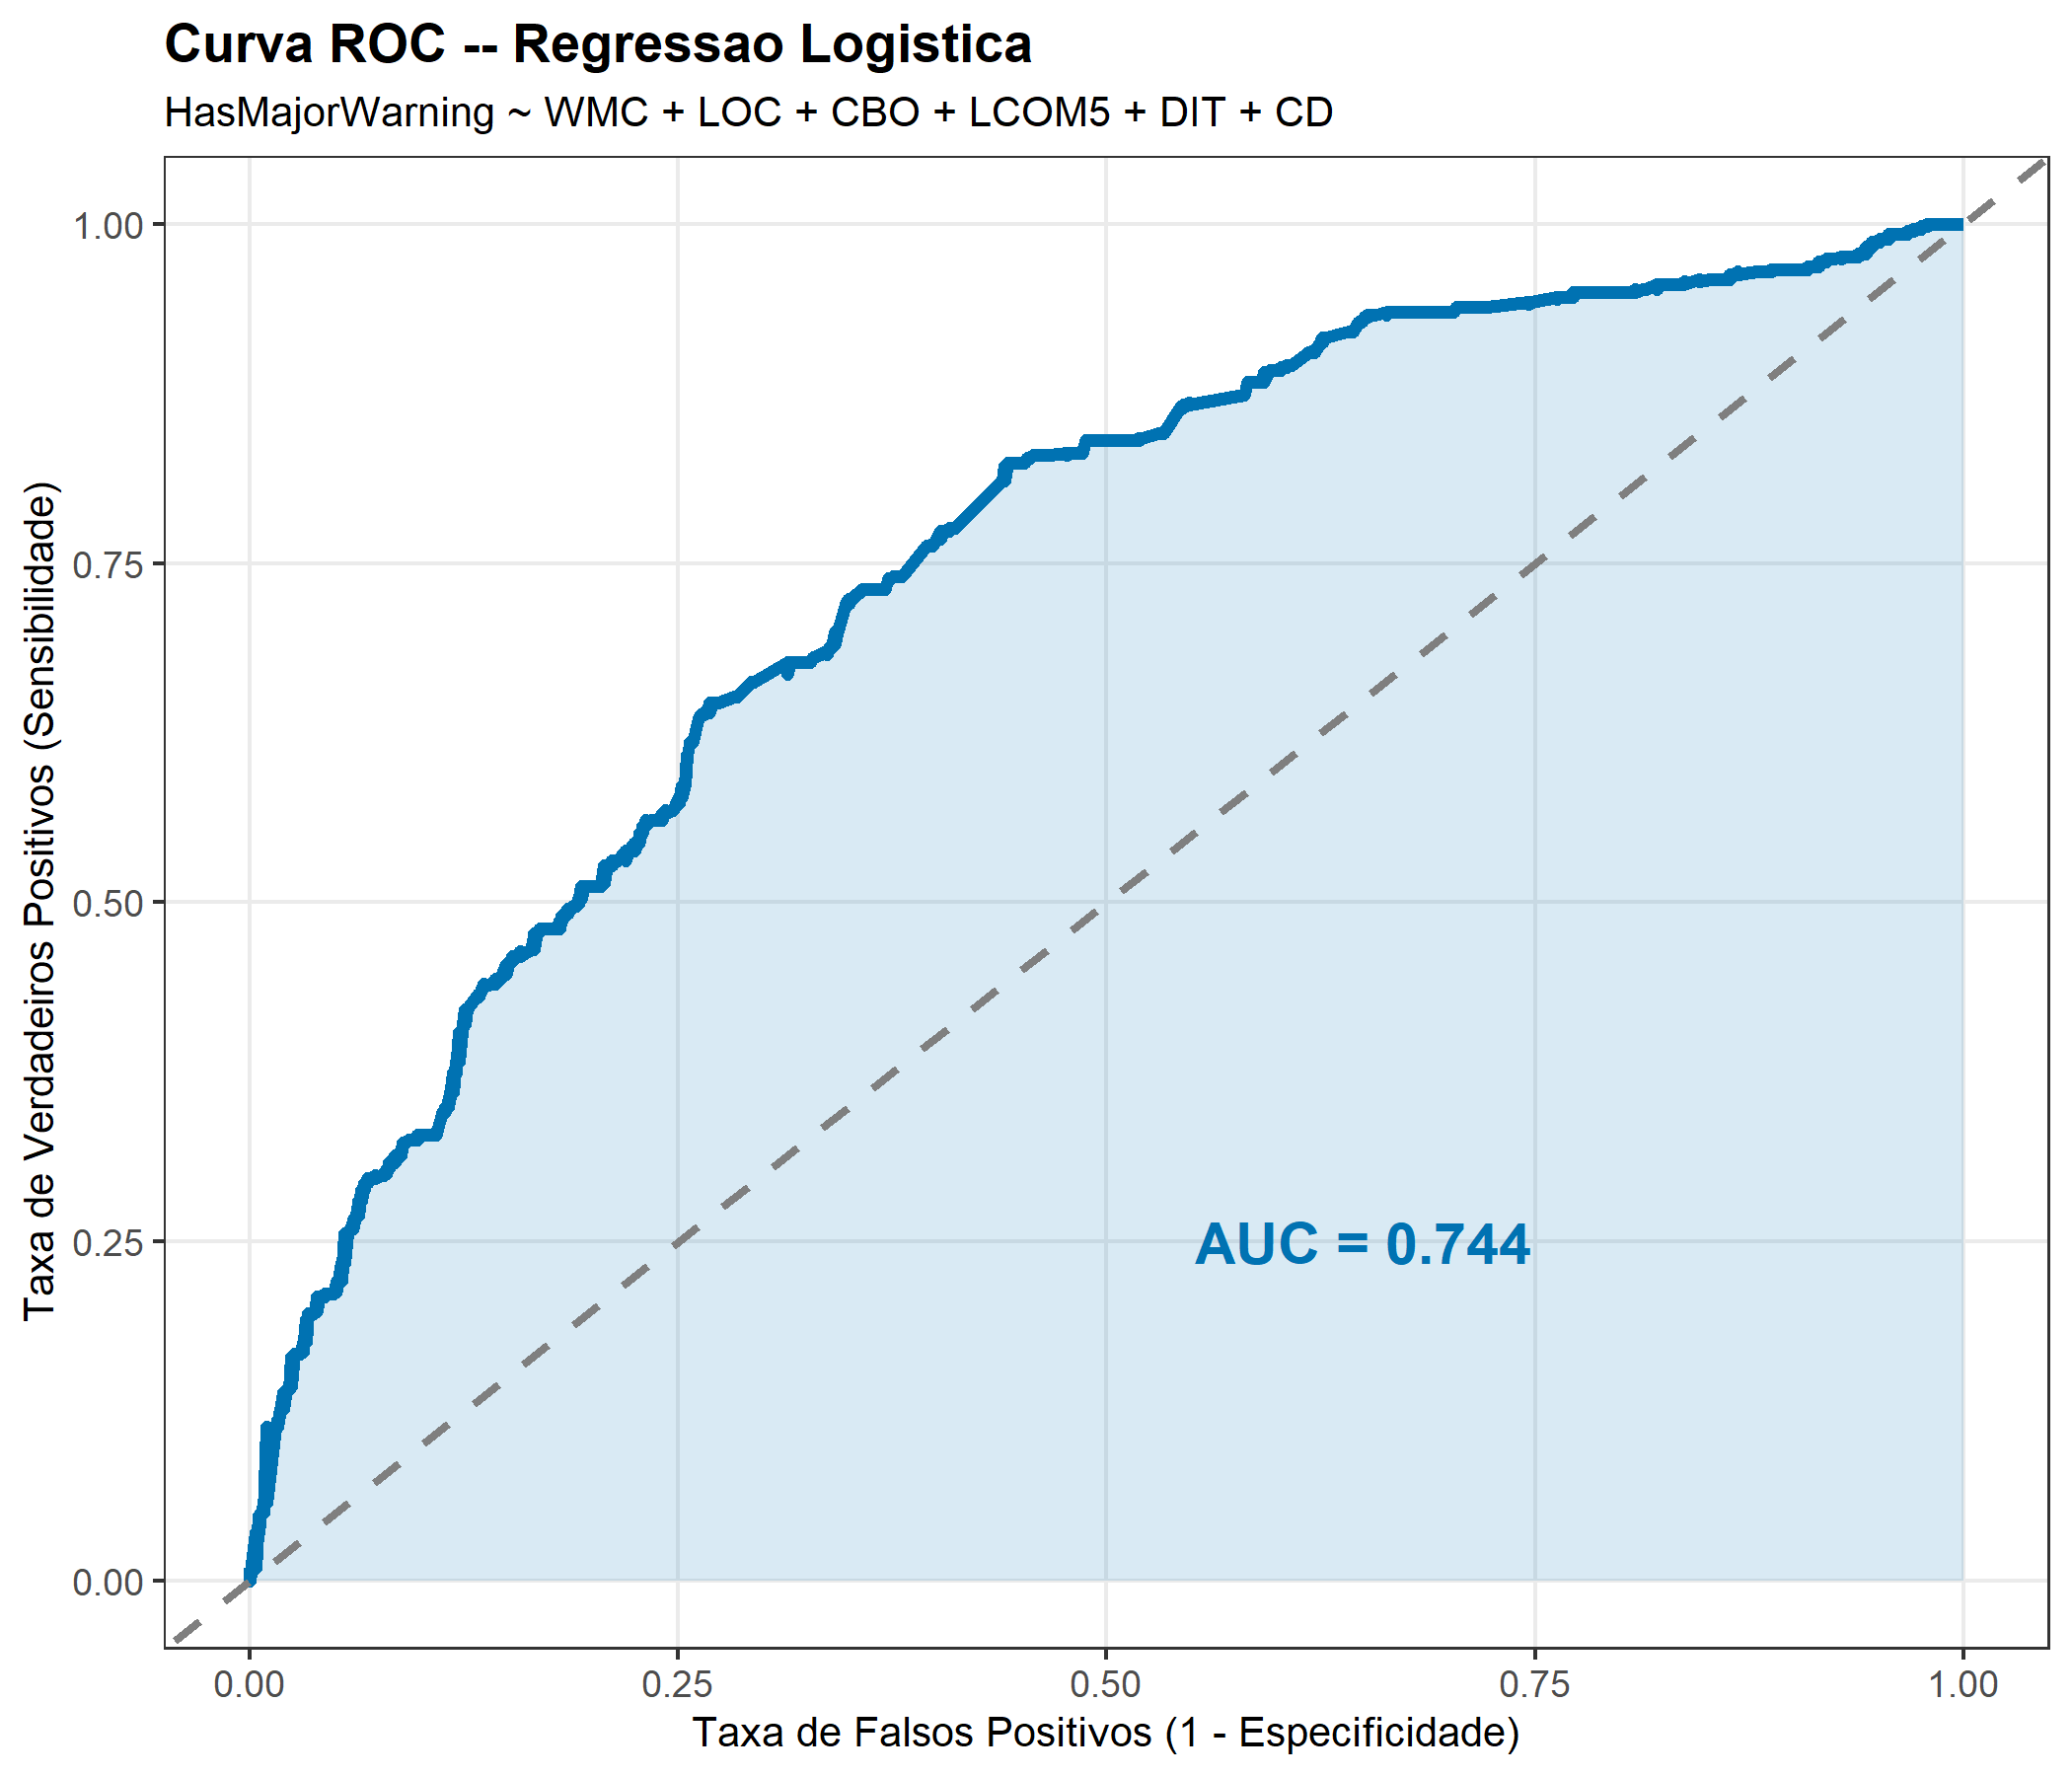
\includegraphics[width=0.60\linewidth]{../output/figures_r/logistic_roc_curve_r.png}
  \caption{Curva ROC do modelo logístico (AUC $= 0{,}744$).}
  \label{fig:roc}
\end{figure}

% ═══════════════════════════════════════════════════════════════
\section{Discussão}
\label{sec:discussao}

\subsection{Cluster Tamanho-Complexidade-Resposta}

A forte correlação entre LOC, WMC e RFC ($r > 0{,}88$) indica que, no
JUnit, essas três métricas medem essencialmente a mesma dimensão: o
``porte'' de uma classe. Classes maiores são automaticamente mais
complexas e expõem mais comportamentos externos. Esse achado é consistente
com a literatura de métricas orientadas a objetos~\cite{chidamber1994}.
Do ponto de vista prático, isso implica que manter classes pequenas é
suficiente para controlar simultaneamente LOC, WMC e RFC.

\subsection{Independência da Herança}

O DIT apresentou correlação próxima de zero com todas as demais variáveis
($|r| < 0{,}1$ com WMC, CBO e LOC). Isso sugere que, no JUnit, a
profundidade da hierarquia de herança não está associada a maior
complexidade ou acoplamento. O framework emprega herança de forma seletiva
e bem encapsulada, sem criar hierarquias profundas que gerem dependências
excessivas.

\subsection{Não-Normalidade e Implicações}

A rejeição universal da normalidade não é uma falha do dataset, mas uma
propriedade fundamental das métricas de software: a distribuição é
determinada pela lei de potência, onde poucas classes grandes dominam
a cauda~\cite{concas2007}. Para estudos comparativos futuros, recomenda-se
o uso de testes não-paramétricos (Mann-Whitney, Kruskal-Wallis) e de
correlação de Spearman, que é mais robusta à assimetria.

\subsection{God Classes}

A análise de outliers identificou classes com LOC muito acima do limite
superior do IQR. \texttt{Assert} (935 LOC, WMC = 96, NM = 67),
\texttt{AssertionTest} (626 LOC, WMC = 108) e \texttt{TestCase} (471 LOC)
são candidatas a \textit{God Classes} — antipadrão que concentra
responsabilidades excessivas em uma única unidade, dificultando
manutenção e teste~\cite{fowler1999}. No contexto de um framework de
testes, essa concentração pode ser justificada pela natureza da API
pública que precisa expor, mas constitui um ponto de atenção para
evoluções futuras.

\subsection{Ausência de Bugs Registrados}

O valor zero na coluna ``\textit{Number of bugs}'' para todas as classes
pode ser interpretado de duas formas: (i)~o JUnit é um software maduro,
amplamente testado e com poucas falhas abertas na versão analisada, ou
(ii)~a metodologia de coleta do dataset pode não ter capturado todos os
bugs. De qualquer forma, a ausência de variabilidade no alvo original
motivou a criação de proxies (WMC e HasMajorWarning) que permitiram
conduzir uma modelagem estatística relevante.

\subsection{Interpretação dos Modelos}

\textbf{Regressão linear:} LCOM5 é o preditor mais relevante
($\beta = 1{,}17$), indicando que classes com menor coesão tendem a
ser mais complexas — resultado intuitivo, pois classes que agrupam
métodos não relacionados tendem a ter mais ramificações lógicas.
NM contribui com $\beta = 0{,}058$ e CBO com $\beta = 0{,}248$:
cada método adicional e cada dependência externa incrementam a
complexidade ponderada. DIT não foi significativo ($p = 0{,}953$),
consistente com sua independência nas correlações.

\textbf{Regressão logística:} LOC aumenta a probabilidade de avisos
PMD severos (OR = 1,027 por linha), LCOM5 quase dobra as chances
(OR = 1,467), enquanto CD as reduz fortemente (OR = 0,175) — classes
bem documentadas tendem a ter menos violações. Esse último resultado
sugere que a prática de comentar o código está associada a um estilo
de desenvolvimento mais cuidadoso.

% ═══════════════════════════════════════════════════════════════
\section{Conclusão}
\label{sec:conclusao}

Este trabalho realizou uma análise estatística abrangente das métricas
de código-fonte do JUnit, cobrindo todas as etapas solicitadas: medidas
de tendência central e dispersão, análise de posição relativa, construção
de gráficos, detecção de outliers, testes de normalidade, análise de
correlação e modelagem estatística.

Os principais achados foram: (i) todas as métricas apresentam forte
assimetria positiva e não-normalidade; (ii) LOC, WMC e RFC formam um
cluster de alta correlação, indicando que porte e complexidade são
dimensões interdependentes no JUnit; (iii) DIT é estatisticamente
independente das demais variáveis, sugerindo uso disciplinado de
herança; (iv) \textit{God Classes} foram identificadas por meio de
análise de outliers; (v) o modelo de regressão linear explica 34\% da
variabilidade de WMC sem recorrer a LOC; e (vi) o modelo logístico
atinge AUC de 0,744 na predição de avisos PMD severos.

Como trabalho futuro, sugere-se: (i) aplicar modelos com transformação
logarítmica para melhorar a homocedasticidade; (ii) investigar modelos
de regressão zero-inflados para as variáveis com alta massa em zero;
(iii) comparar os resultados com outros frameworks da base (Neo4j,
Elasticsearch) para verificar generalidade dos padrões encontrados.

% ═══════════════════════════════════════════════════════════════
\bibliographystyle{sbc}
\bibliography{references}

\end{document}
